\section{Operations on Tensors}\label{chapter:operations}
Recall that a tensor $\Tt \in \RR^{d_1 \times \cdots \times d_N}$ can be seen as a multi-dimensional array of order $N$: an $N$-th order or $N$-way tensor has $N$ modes, each mode corresponding to one dimension \citep{kolda2009tensor}.
\paragraph{Tensor Fibers} For any mode-$i$ (where $i = 1, \dots, N$), tensor \textit{fibers} are obtained by keeping all indices fixed except the $i$-th one. For example, a matrix column corresponds to a mode-1 fiber, while a matrix row corresponds to a mode-2 fiber. In a third-order tensor $\Tt \in \RR^{d_1 \times d_2 \times d_3}$, we have $d_2d_3$ mode-1 fibers, which are vectors of size $d_1$, i.e., $\Tt_{:,i_2,i_3} \in \RR^{d_1}$ for $i_2 \in [d_2]$ and $i_3 \in [d_3]$. The colon indicates varying the first index, while $i_2$ and $i_3$ remain fixed. Fibers are vectors.
\paragraph{Tensor Slices} Slices of a tensor are two-dimensional arrays (matrices) obtained by fixing all but two indices. For a third-order tensor $\Tt \in \RR^{d_1 \times d_2 \times d_3}$, there are horizontal, lateral, and frontal slices denoted by $\Tt_{i_1,:,:} \in \RR^{d_2 \times d_3}$, $\Tt_{:,i_2,:} \in \RR^{d_1 \times d_3}$, and $\Tt_{:,:,i_3} \in \RR^{d_1 \times d_2}$, respectively. Therefore, slices are matrices.
\paragraph{Scalar Multiplication} 
Let $\lambda \in \RR$ be a scalar. The scalar product $\lambda\Tt$ 
 is a tensor of the same dimension $d_1 \times \cdots \times d_N$, defined element-wise by:
$
    (\lambda\Tt)_{i_1 \cdots i_N} = \lambda \cdot \Tt_{i_1 \cdots i_N}$
for all admissible indices $i_k\in[d_k]$ and $k\in[N]$.
\paragraph{Tensors Sum} Let $\St\in\RR^{d_1\times\cdots\times d_N}$. The sum of tensors $\Tt$ and $\St$ is a tensor of the same dimension, $\Tt+\St\in\RR^{d_1\times\cdots\times d_N}$, defined element-wise by: $(\Tt+\St)_{i_1,\cdots,i_N} = \Tt_{i_1,\cdots,i_N} + \St_{i_1,\cdots,i_N}$ for all admissible indices $i_k\in[d_k]$ and $k\in[N]$.
\subsection{Permute and Reshape Tensors}
Permutation and reshaping are two fundamental operations on tensors.
\begin{itemize}
    \item \textbf{Permutation} rearranges the indices of a tensor without changing its number of modes. A common example of a permutation is the transpose of a matrix.
    \item  \textbf{Reshaping} combines multiple indices into larger ones or divides a large index into multiple smaller indices, reducing or increasing the total number of indices while preserving the overall size of the tensor.
\end{itemize}
We introduce matricization and vectorization, two common reshaping operations on tensors.
\begin{definition}(Matricization)\label{matricizitation:def}
Let $\Tt\in\RR^{d_1\times d_2\times \cdots\times d_N}$. The mode-$n$ matricization  $\Tt_{(n)}\in\RR^{d_n\times d_1d_2\cdots d_{n-1}d_{n+1}\cdots d_N}$, for $n\in[N]$, is obtained by unfolding $\Tt$ into a matrix by taking all mode-$n$ fibers and stacking them as columns. For example, the matricization of a tensor $\Tt\in\RR^{d_1\times d_2\times d_3}$ along mode-$1$, which is denoted by $\Tt_{(1)}$, is the $d_1\times d_2d_3$ matrix
$$
    \begin{bmatrix}
    \vline & \vline & \vline  & \vline \\
    \Tt_{:,1,1} & {\Tt}_{:,1,2}  & \dots  & {\Tt}_{:,d_2,d_3} \\
    \vline & \vline & \vline  & \vline 
    \end{bmatrix}
\in\RR^{d_1\times d_2d_3}.
$$

The mode-2 and mode-3 matricizations $\Tt_{(2)}\in\RR^{d_2\times d_1d_3}$ and $\Tt_{(3)}\in\RR^{d_3\times d_1d_2}$ are defined similarly.
\end{definition}

Observe that in mode-1 matricization, the two indices corresponding to the second and third modes of $\Tt$ are grouped together to form a new index that ranges from 1 to $d_2d_3$. In the previous definition, we chose to order this new index using lexicographic ordering, e.g., $11,12,13,21,22,23,31,32,33$ if $d_2=d_3=3$. Different orderings of the columns for matricizations are sometimes used~(e.g., reverse lexicographic in \citep{kolda2009tensor}). In general, the specific ordering
used is not important, but it must be consistent across related calculations~(see \citep{kolda2006multilinear} for further details).



In tensor network diagrams, we represent such a grouping of indices by merging the corresponding legs together:
$$\Tt_{(1)} = 
\left(\begin{tikzpicture}[baseline=\baseline]
    \tikzset{tensor/.style = {minimum size = 0.5cm,shape = circle,thick,draw=black,inner sep = 0pt}, edge/.style = {thick,line width=.4mm},every loop/.style={}}
    \def\y{0}
    \def\x{0}
    \node[tensor,fill=red!50!white] (T) at (\x,\y){\scalebox{0.85}{$\Tt$}};
    \draw[edge] (T) -- (\x+0.7,\y) node [midway,above]{\scalebox{0.7}{\dimcolor{$d_2$}}};
    \draw[edge] (T) -- (\x-0.7,\y) node [midway,above]{\scalebox{0.7}{\dimcolor{$d_1$}}};
    \draw[edge] (T) -- (\x,\y-0.7) node [midway,left]{\scalebox{0.7}{\dimcolor{$d_3$}}}; 
\end{tikzpicture}\right)_{(1)}
=
\begin{tikzpicture}[baseline=\baseline]
    \tikzset{tensor/.style = {minimum size = 0.5cm,shape = circle,thick,draw=black,inner sep = 0pt}, edge/.style = {thick,line width=.4mm},every loop/.style={}}
    \def\y{0}
    \def\x{0}
    \node[tensor,fill=red!50!white] (A) at (\x,\y){\scalebox{0.85}{$\Tt$}};
    \draw[edge] (\x+0.2,\y+0.15) -- (\x+0.5,\y+0.15)-- (\x+0.5,\y+0.05) -- (\x+1,\y+0.05) node [midway,above]
    {\scalebox{0.7}{\dimcolor{$d_2$}}};
    \draw[edge] (\x+0.2,\y-0.15) -- (\x+0.5,\y-0.15)-- (\x+0.5,\y-0.05)-- (\x+1,\y-0.05) node [midway,below]
    {\scalebox{0.7}{\dimcolor{$d_3$}}};
    \draw[edge] (A) -- (\x-0.7,\y)node [midway,above]
    {\scalebox{0.7}{\dimcolor{$d_1$}}};
\end{tikzpicture}
=
\begin{tikzpicture}[baseline=\baseline]
    \tikzset{tensor/.style = {minimum size = 0.5cm,shape = circle,thick,draw=black,inner sep = 0pt}, edge/.style = {thick,line width=.4mm},every loop/.style={}}
    \def\y{0}
    \def\x{0}
    \node[tensor,fill=red!50!white] (T) at (\x,\y){\scalebox{0.85}{$\Tt$}};
    \draw[edge](T) -- (\x+1,\y) node [midway, above]{\scalebox{0.7}{\dimcolor{$d_2d_3$}}};
    \draw[edge](T) -- (\x-1,\y) node [midway, above]{\scalebox{0.7}{\dimcolor{$d_1$}}};
\end{tikzpicture}
\in\RR^{d_1\times d_2d_3}.
$$
As we can see, the grouped legs of the shape
$\begin{tikzpicture}[baseline=\baseline]
    \tikzset{tensor/.style = {minimum size = 0.5cm,shape = circle,thick,draw=black,inner sep = 0pt}, edge/.style = {thick,line width=.4mm},every loop/.style={}}
    \def\y{0}
    \def\x{0}
    \draw[edge] (\x+0.15,\y+0.2) -- (\x+0.5,\y+0.2) -- (\x+0.5,\y+0.1) -- (\x+1,\y+0.1) node [midway,above]
    {\scalebox{0.7}{\dimcolor{$d_2$}}};
    \draw[edge] (\x+0.15,\y-0.1) -- (\x+0.5,\y-0.1)-- (\x+0.5,\y)-- (\x+1,\y) 
node [midway,below]
    {\scalebox{0.7}{\dimcolor{$d_3$}}};
    \end{tikzpicture}
$
represents an edge of size $d_2d_3$ in tensor network diagrams.


In general, the notion of matricization can be extended to any subset $I\subset [N]$ of the modes of $\Tt$ which map  modes in $I$  to rows and the modes not in $I$ to columns, resulting in a matrix $\Tt_{(I)}$ of size $\prod_{i\in I} d_i \times \prod_{j\in [N]\setminus I} d_j$. For instance, for a sixth-order tensor $\Tt\in\RR^{d_1\times\dots\times d_6}$ we can group the indices as follows:
\begin{align*}
\Tt_{i_1,\dots,i_6} 
&=
\begin{tikzpicture}[baseline=\baseline]
    \tikzset{tensor/.style = {minimum size = 0.5cm,shape = circle,thick,draw=black,inner sep = 0pt}, edge/.style = {thick,line width=.4mm},every loop/.style={}}
    \def\y{0}
    \def\x{0}
    \node[tensor,fill=red!20!blue!40!white] (T) at (\x,\y){\scalebox{0.85}{$\Tt$}};
    \draw[edge] (T) -- (\x+0.85,\y) node [very near end,right]
    {\scalebox{0.7}{\indcolor{$i_4$}}};
    \draw[edge] (T) -- (\x,\y-0.85) node [very near end, below]
    {\scalebox{0.7}{\indcolor{$i_6$}}};
    \draw[edge] (T) -- (\x-0.85,\y)node [very near end,left]
    {\scalebox{0.7}{\indcolor{$i_1$}}};
    \draw[edge] (T) -- (\x,\y+0.85) node [very near end,above]
    {\scalebox{0.7}{\indcolor{$i_3$}}};
    \draw[edge] (T) -- (\x-0.75,\y+0.5) node [pos=1.3]
    {\scalebox{0.7}{\indcolor{$i_2$}}};
    \draw[edge] (T) -- (\x+0.75,\y-0.5) node [pos=1.3]
    {\scalebox{0.7}{\indcolor{$i_5$}}};
    \node[draw=none] at (\x+2,\y+0.2){$\underrightarrow{I=\{1,2,6\}}$};
    \end{tikzpicture}
\begin{tikzpicture}[baseline=\baseline]
    \tikzset{tensor/.style = {minimum size = 0.5cm,shape = circle,thick,draw=black,inner sep = 0pt}, edge/.style = {thick,line width=.4mm},every loop/.style={}}
    \def\y{0}
    \def\x{0}
    \node[tensor,fill=red!20!blue!40!white] (T) at (\x,\y){\scalebox{0.85}{$\Tt$}};
    \draw[edge](T) -- (\x+0.85,\y)node [very near end, right]{\scalebox{0.7}{\indcolor{$i_5$}}};
    \draw[edge](\x+0.16,\y+0.2) -- (\x+0.5,\y+0.2) -- (\x+0.5,\y+0.1) -- (\x+0.85,\y+0.1)node [very near end, above]{\scalebox{0.7}{\indcolor{$i_3$}}};
    \draw[edge](\x+0.16,\y-0.2) -- (\x+0.5,\y-0.2) -- (\x+0.5,\y-0.1) -- (\x+0.85,\y-0.1)node [very near end, below]{\scalebox{0.7}{\indcolor{$i_4$}}};
    \draw[edge](T) -- (\x-0.85,\y)node [very near end, left]{\scalebox{0.7}{\indcolor{$i_2$}}};
    \draw[edge](\x-0.16,\y+0.2) -- (\x-0.5,\y+0.2) -- (\x-0.5,\y+0.1) -- (\x-0.85,\y+0.1)node [very near end, above]{\scalebox{0.7}{\indcolor{$i_6$}}};
    \draw[edge](\x-0.16,\y-0.2) -- (\x-0.5,\y-0.2) -- (\x-0.5,\y-0.1) -- (\x-0.85,\y-0.1)node [very near end, below]{\scalebox{0.7}{\indcolor{$i_1$}}};
\end{tikzpicture}\\
&=
(\Tt_{(\{1,2,6\})})_{i_1i_2i_6 , i_3i_4i_5}\in\RR^{d_1d_2d_6\times d_3d_4d_5}.
\end{align*}
While this concept is intuitive, it is clunky to write formally: the indices $i_{r_1},i_{r_2},\cdots, i_{r_{|I|}}$ in $I$ (decreasingly ordered) of a tensor are mapped to the row index $
j = 1+\sum_{l=1}^{|I|}
\left[(i_{r_l}-1)\prod_{m=1}^{l-1}I_{r_m}\right]
$, while the remaining indices $i_{c_1},i_{c_2},\cdots, i_{c_{N-|I|}}$ (again decreasingly ordered) are mapped to the column index $k  = 1+\sum_{n=1}^{N - |I|}
\left[(i_{c_n}-1)\prod_{s=1}^{n-1}I_{r_s}\right]$. Using tensor networks allows us to abstract away this clunkiness by simply representing such 
reshaping operations by grouping legs together. 






Likewise, just as a tensor can be converted into a matrix, it can also be converted into a vector. This process is called vectorization:
\begin{definition}(Vectorization)\label{def:vectorization}
Let $\Tt\in\RR^{d_1\times d_2\times\cdots\times d_N}$. The \emph{vectorization} of $\Tt$ denoted as $\vectorize(\Tt)\in\RR^{d_1d_2\cdots d_N}$ is the vector obtained by concatenating its mode-$N$ fibers\footnote{Using the lexicographic order.}. For example, the vectorization of a tensor $\Tt\in\RR^{d_1\times d_2\times d_3}$ is given by:
$$\vectorize(\Tt) =    
[(\Tt_{1,1,:})\ \  (\Tt_{1,2,:})\ \  \cdots \ \ (\Tt_{d_1,d_2,:})]^\ts
=
\begin{tikzpicture}[baseline=\baseline]
    \tikzset{tensor/.style = {minimum size = 0.5cm,shape = circle,thick,draw=black,inner sep = 0pt}, edge/.style = {thick,line width=.4mm},every loop/.style={}}
    \def\y{0}
    \def\x{0}
    \node[tensor,fill=blue!10!white] (A) at (\x,\y){\scalebox{0.85}{$\Tt$}};
    \draw[edge] (\x+0.15,\y+0.2) -- (\x+0.5,\y+0.2) -- (\x+0.5,\y+0.1) -- (\x+1,\y+0.1) node [midway,above]
    {\scalebox{0.7}{\dimcolor{$d_1$}}};
     \draw[edge] (A) -- (\x+1,\y)node [right]
    {\scalebox{0.7}{\dimcolor{$d_2$}}};

    \draw[edge] (\x+0.15,\y-0.2) -- (\x+0.5,\y-0.2)-- (\x+0.5,\y-0.1)-- (\x+1,\y-0.1) node [midway,below]
    {\scalebox{0.7}{\dimcolor{$d_3$}}};
    \end{tikzpicture}\in\RR^{d_1d_2d_3}.
$$
\end{definition}

Vectorization is a flattening operation that converts a tensor of any order into a vector. Similarly to matricization, in tensor networks
the edge of the shape $
\begin{tikzpicture}[baseline=\baseline]
    \tikzset{tensor/.style = {minimum size = 0.5cm,shape = circle,thick,draw=black,inner sep = 0pt}, edge/.style = {thick,line width=.4mm},every loop/.style={}}
    \def\y{0}
    \def\x{0}
    \draw[edge] (\x+0.15,\y+0.2) -- (\x+0.5,\y+0.2) -- (\x+0.5,\y+0.1) -- (\x+1,\y+0.1) node [midway,above]
    {\scalebox{0.7}{\textcolor{gray}{$d_1$}}};
    \draw[edge] (\x+0.15,\y) -- (\x+1,\y)node [right]
    {\scalebox{0.7}{\textcolor{gray}{$d_2$}}};
    \draw[edge] (\x+0.15,\y-0.2) -- (\x+0.5,\y-0.2)-- (\x+0.5,\y-0.1)-- (\x+1,\y-0.1) 
node [midway,below]
    {\scalebox{0.7}{\dimcolor{$d_3$}}};
    \end{tikzpicture}
$ represents an edge of size $d_1d_2d_3$. In general, throughout this manuscript, convergent edges represent an edge whose size is the product of the sizes of all associated edges. Note that the vectorization of a tensor is equal to the vectorization\footnote{To be consistent with the definition of vectorization used in this book, the vectorization of a matrix is given by the concatenation of its rows, which is sometimes referred to as \emph{row-major vectorization}.Note that this is the default vectorizing operation, \textsf{ravel()}, of the \textsf{numpy} package in \textsf{Python}.} of the  mode-$1$ matricization of the tensor, i.e., for $\Tt\in\RR^{d_1\times d_2\cdots \times d_N}$, $\vectorize(\Tt) = \vectorize(\Tt_{(1)})$.




\subsection{Products}\label{sec:product}
Tensors can be combined or \textit{multiplied} using different types of operation. In this section, we provide graphical illustrations of different product operations.
\paragraph{Mode-$n$ Tensor Product}\label{par:mode-n-tensor-product}
The modes $n$ products, where a tensor is multiplied by a matrix along a specific mode, can be seen as a generalization of the matrix products. More precisely, the mode-$n$ product generalizes matrix-matrix multiplication along one particular mode. These include mode-$n$ products between tensors and matrices, as well as tensors and vectors.
\begin{enumerate}
\item \textbf{Mode-n product~(matrix).}\label{subsec:mode-n}
    The mode-$n$ product of a tensor $\Xt\in\RR^{d_1\times\cdots\times d_N}$ with a matrix $\Mb\in\RR^{m\times d_n}$ denoted as
    $\Xt\ttm n \Mb \in \RR^{d_1\times \cdots\times d_{n-1}\times m\times d_{n+1}\times\cdots\times d_N}$ is defined as the contraction of a tensor with a matrix along mode-$n$ of the tensor and mode-2 of the matrix~(column index), i.e., 
    $$
  \Xt\ttm n \Mb
=
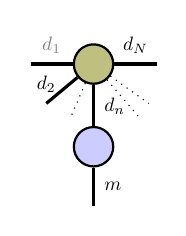
\begin{tikzpicture}[baseline=-0.5ex]
    \tikzset{tensor/.style = {minimum size = 0.5cm,shape = circle,thick,draw=black,inner sep = 0pt}, edge/.style = {thick,line width=.4mm},every loop/.style={}}
    \def\x{6}
    \node[tensor,fill=blue!20!white] (M) at (\x,-1.05) {$\Mb$};
    \node[tensor,fill=green!50!red!50!white] (At) at (\x,0) {$\Xt$};
    \draw[edge] (At) -- (\x-0.8,0) node [midway,above] {\scalebox{0.7}{\textcolor{gray}{$d_1$}}};
    \draw[edge] (At)-- (\x-0.6,-0.5) node [above]{\scalebox{0.7}{\dimcolor{$d_2$}}};
    \draw[edge] (At) -- (\x+0.8,0) node [midway,above] {\scalebox{0.7}{\dimcolor{$d_N$}}};;
    \draw[dotted] (At) -- (\x-0.3,-0.7);
    \draw[edge] (At) -- (\x,-0.8) node [midway,right] {\scalebox{0.7}{\dimcolor{$d_n$}}};
    \draw[dotted] (At) -- (\x+0.6,-0.7);
    \draw[dotted] (At) -- (\x+0.7,-0.5);
    \draw[edge] (M) -- (\x,-1.8) node [midway,right] {\scalebox{0.7}{\dimcolor{$m$}}};;
    \end{tikzpicture}
\in\RR^{d_1\times  \dots\times d_{n-1}\times m \times d_{n+1}\times \dots\times d_N}.
$$
The operation contracts the tensor's $n$-th mode with the matrix's second mode~(column), replacing the original dimension $d_n$ with a new dimension $m$. For $\Ab\in\RR^{d_n\times n},\Bb\in\RR^{d_m\times m}$ and $\Xt\in\RR^{d_1\times\cdots\times d_N}$ with distinct modes $n\neq m$, the order of multiplication does not matter, i.e.,
$$
\Xt\ttm n \Ab \ttm m \Bb = 
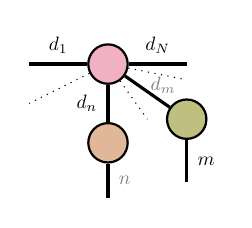
\begin{tikzpicture}[baseline=-0.5ex]
    \tikzset{tensor/.style = {minimum size = 0.5cm,shape = circle,thick,draw=black,inner sep = 0pt}, edge/.style = {thick,line width=.4mm},every loop/.style={}}
    \def\x{0}
    \def\y{0}
    \node[tensor,fill=blue!20!red!30!white] (Xt) at (\x,\y) {$\Xt$};
    \node[tensor,fill=green!30!red!40!white] (A) at (\x,\y-1) {$\Ab$};
    \node[tensor,fill=green!50!red!50!white] (B) at (\x+1,\y-0.7) {$\Bb$};
    \draw[edge] (Xt) -- (\x-1,\y) node [midway,above] {\scalebox{0.7}{\dimcolor{$d_1$}}};
    \draw[dotted] (Xt) -- (\x-1,\y-0.5);
    \draw[edge] (Xt) -- (\x+1,\y) node [midway,above] {\scalebox{0.7}{\dimcolor{$d_N$}}};
    \node[draw=none] () at (\x+0.7,\y-0.27) {\scalebox{0.7}{\textcolor{gray}{$d_m$}}};
    \draw[edge] (Xt) -- (A) node [midway,left] {\scalebox{0.7}{\dimcolor{$d_n$}}};
    \draw[edge] (A) -- (\x,\y-1.7) node [midway,right] {\scalebox{0.7}{\textcolor{gray}{$n$}}};
    \draw[edge] (Xt) -- (B);
    \draw[edge] (B) -- (\x+1,\y-1.5) node [midway,right] {\scalebox{0.7}{\dimcolor{$m$}}};
    \draw[dotted] (Xt) -- (\x+1,\y-0.2);
    \draw[dotted] (Xt) -- (\x+0.5,\y-0.7);
    \end{tikzpicture}
= \Xt\ttm m\Bb\ttm n \Ab,~~\text{For}~~n\neq m.
$$
However, if $m = n$ the order of the products is important. In particular, if $\Ab\in\RR^{n\times d_n}$ and $\Bb\in\RR^{p\times n}$ we have $(\Xt\ttm n \Ab) \ttm n \Bb = \Xt\ttm n(\Bb\Ab)$, whereas the product $(\Xt\ttm n \Bb) \ttm n \Ab$ is not valid unless $n=d_n=p$.
The mode-$n$ tensor product can be seen as a generalization of classical matrix multiplication. In particular,
we can recover matrix products with mode-$1$ and mode-$2$ products of an order 2 tensor: 
if $\Ab\in\RR^{m\times n}$, $\Bb\in\RR^{p\times n}$ and $\Cb\in\RR^{d\times m}$, then
\begin{align*}
\Ab\ttm2 \Bb
=
\begin{tikzpicture}[baseline=\baseline]
   \tikzset{tensor/.style = {minimum size = 0.5cm,shape = circle,thick,draw=black,inner sep = 0pt}, edge/.style = {thick,line width=.4mm},every loop/.style={}}
    \def\y{0}
    \def\x{0}
    \node[tensor,fill=red!50!white] (A) at (\x,\y){\scalebox{0.85}{$\Ab$}};
    \node[tensor,fill=blue!50!white] (B) at (\x+1,\y){\scalebox{0.85}{$\Bb$}};
    \draw[edge] (A) -- (B) node [above,midway] {\scalebox{0.7}{\dimcolor{$n$}}};
    \draw[edge] (\x-0.25,\y) -- (\x-0.6,\y)  node [midway,above] {\scalebox{0.7}{\dimcolor{$m$}}};
    \draw[edge] (\x+1.25,\y) -- (\x+1.6,\y)  node [midway,above] {\scalebox{0.7}{\dimcolor{$p$}}};
    \end{tikzpicture}
    = \Ab\Bb^\ts\in\RR^{m\times p},
\end{align*}
\begin{align*}
    \Ab\ttm1 \Cb =
    \begin{tikzpicture}[baseline=\baseline]
   \tikzset{tensor/.style = {minimum size = 0.5cm,shape = circle,thick,draw=black,inner sep = 0pt}, edge/.style = {thick,line width=.4mm},every loop/.style={}}
    \def\y{0}
    \def\x{0}
    \node[tensor,fill=red!20!white] (C) at (\x,\y){\scalebox{0.85}{$\Cb$}};
    \node[tensor,fill=red!50!white] (A) at (\x+1,\y){\scalebox{0.85}{$\Ab$}};
    \draw[edge] (C) -- (A) node [above,midway] {\scalebox{0.7}{\dimcolor{$m$}}};
    \draw[edge] (\x-0.25,\y) -- (\x-0.6,\y)  node [midway,above] {\scalebox{0.7}{\dimcolor{$d$}}};
    \draw[edge] (\x+1.25,\y) -- (\x+1.6,\y)  node [midway,above] {\scalebox{0.7}{\dimcolor{$n$}}};
    \end{tikzpicture}
    = \Cb\Ab\in\RR^{d\times n}.
\end{align*}

We show in the following proposition how the mode-$n$ product can be expressed through matricization and matrix product. 
\begin{proposition}
Let $\Xt\in\RR^{d_1\times\dots\times d_N}$ and $\Mb\in\RR^{m\times d_n}$ then 
$(\Xt\ttm n \Mb)_{(n)} = \Mb\Xt_{(n)}$.
\begin{proof}
We show this identity with a simple tensor network diagram for the special case $n=2$ and $N=3$. The extension to the general case is straightforward. We have
\begin{align*}
(\Xt\ttm2\Mb)_{(2)} 
&= 
\left(
    \begin{tikzpicture}[baseline=\baseline]
    \tikzset{tensor/.style = {minimum size = 0.5cm,shape = circle,thick,draw=black,inner sep = 0pt}, edge/.style = {thick,line width=.4mm},every loop/.style={}}
    \def\y{0}
    \def\x{0}
    \node[tensor,fill=green!50!red!50!white] (At) at (\x,\y){\scalebox{0.85}{$\Xt$}};
    \node[tensor,fill=blue!20!white] (M) at (\x-1,\y) {$\Mb$};
    \draw[edge] (At) -- (M) node [midway,above]
    {\scalebox{0.7}{\dimcolor{$d_2$}}};
    \draw[edge] (M) -- (\x-1.7,\y) node [midway,above]
    {\scalebox{0.7}{\dimcolor{$m$}}};);
    \draw[edge] (At)-- (\x+0.5,\y+0.5) node [below] {\scalebox{0.7}{\dimcolor{$d_1$}}};
    \draw[edge] (At)-- (\x+0.5,\y-0.5) node [above] {\scalebox{0.7}{\dimcolor{$d_3$}}};
    \end{tikzpicture}
\right)_{(2)}
=
    \begin{tikzpicture}[baseline=\baseline]
    \tikzset{tensor/.style = {minimum size = 0.5cm,shape = circle,thick,draw=black,inner sep = 0pt}, edge/.style = {thick,line width=.4mm},every loop/.style={}}
    \def\y{0}
    \def\x{0}
    \node[tensor,fill=green!50!red!50!white] (At) at (\x,\y){\scalebox{0.85}{$\Xt$}};
    \node[tensor,fill=blue!20!white] (M) at (\x-1,\y) {$\Mb$};
    \draw[edge] (At) -- (M) node [midway,above]
    {\scalebox{0.7}{\dimcolor{$d_2$}}};
    \draw[edge] (M) -- (\x-1.7,\y) node [midway,above]
    {\scalebox{0.7}{\dimcolor{$m$}}};);
    \draw[edge] (\x+0.15,\y+0.2)-- (\x+0.5,\y+0.2)-- (\x+0.5,\y+0.05) -- (\x+1,\y+0.05) node [above] {\scalebox{0.7}{\dimcolor{$d_1$}}};
    \draw[edge] (\x+0.15,\y-0.2) -- (\x+0.5,\y-0.2)--(\x+0.5,\y-0.04)--(\x+1,\y-0.04) node [below] {\scalebox{0.7}{\dimcolor{$d_3$}}};
    \end{tikzpicture}\\
&=
\Mb\Xt_{(2)} \in\RR^{m\times d_1d_3}.
\end{align*}
\end{proof}
\end{proposition}
\item\textbf{Mode-n product~(vector).} The mode-$n$ product of a tensor $\Xt\in\RR^{d_1\times\cdots\times d_N}$ with a vector $\vb\in\RR^{d_n}$, is denoted by 
$\Xt \ttm n \vb \in\RR^{d_1\times\cdots \times d_{n-1}\times d_{n+1}\times \cdots\times d_N}$. Note that the result is a tensor of order $N-1$. It can be pictured in a tensor network diagram as 
    $$
\Xt\ttm n \vb
=
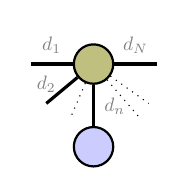
\begin{tikzpicture}[baseline=-0.5ex]
    \tikzset{tensor/.style = {minimum size = 0.5cm,shape = circle,thick,draw=black,inner sep = 0pt}, edge/.style = {thick,line width=.4mm},every loop/.style={}}
    \def\x{6}
    \node[tensor,fill=blue!20!white] (M) at (\x,-1.05) {$\vb$};
    \node[tensor,fill=green!50!red!50!white] (At) at 
    (\x,0) {$\Xt$};
    \draw[edge] (At) -- (\x-0.8,0) node [midway,above] {\scalebox{0.7}{\textcolor{gray}{$d_1$}}};
    \draw[edge] (At)-- (\x-0.6,-0.5) node [above]{\scalebox{0.7}{\textcolor{gray}{$d_2$}}};
    \draw[edge] (At) -- (\x+0.8,0) node [midway,above] {\scalebox{0.7}{\textcolor{gray}{$d_N$}}};;
    \draw[dotted] (At) -- (\x-0.3,-0.7);
    \draw[edge] (At) -- (\x,-0.8) node [midway,right] {\scalebox{0.7}{\textcolor{gray}{$d_n$}}};
    \draw[dotted] (At) -- (\x+0.6,-0.7);
    \draw[dotted] (At) -- (\x+0.7,-0.5);
    \end{tikzpicture}
\in\RR^{d_1\times  \dots\times d_{n-1}\times d_{n+1}\times \dots\times d_N}.
$$
Note that in mode-$n$ vector multiplication, unlike mode-$n$ matrix multiplication, the order of multiplication matters as a vector contraction reduces the tensor order by 1, so subsequent mode indices shift. Let $\Xt\in\RR^{d_1\times\cdots\times d_m\times\cdots\times d_n\times\cdots\times d_N}$ and $\ab\in\RR^{d_n},\bb\in\RR^{d_m}$, then
$
\Xt\ttm n \ab\ttm m\bb \neq
(\Xt \ttm m \bb)\ttm{n}\ab,
$
as mode-$n$ vector multiplication drops the $m$-th dimension~\citep{bader2006algorithm}.
\end{enumerate}







Next, we introduce several important products that are often used in tensor derivations: Kronecker, Khatri-Rao, and Hadamard products.

\paragraph{Kronecker product}\label{subsection-kron}
Let $\Ab\in\RR^{m\times n}$ and $\Bb\in\RR^{p\times q}$. The Kronecker product, $\Ab\kron\Bb\in\RR^{mp\times nq}$ is defined by
\begin{align}
    \Ab\kron\Bb = 
    \begin{bmatrix}
    a_{11}\Bb & a_{12}\Bb & \dots & a_{1n}\Bb \\
    a_{21}\Bb & a_{22}\Bb & \dots & a_{2n}\Bb \\
    \vdots & \vdots & \ddots & \vdots \\
    a_{m1}\Bb & a_{m2}\Bb & \dots & a_{mn}\Bb 
    \end{bmatrix}.
\end{align}

In tensor networks, the Kronecker product is given by the following diagram:
\begin{align}
    \Ab\kron\Bb = 
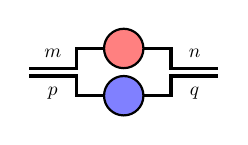
\begin{tikzpicture}[baseline=-0.5ex]
    \tikzset{tensor/.style = {minimum size = 0.5cm,shape = circle,thick,draw=black,inner sep = 0pt}, edge/.style   = {thick,line width=.4mm}}
    \def\x{0}
    \def\y{0}
    \node[tensor,fill=red!50!white] (A) at (\x,\y+0.3){$\Ab$};
    \node[tensor,fill=blue!50!white] (B) at (\x,\y-0.3){$\Bb$};
    \draw[edge] (\x-0.25,\y+0.3) -- (\x-0.6,\y+0.3) -- (\x-0.6,\y+0.05)   -- (\x-1.2,\y+0.05) node [midway,above] {\scalebox{0.7}{\dimcolor{$m$}}};
    \draw[edge] (\x-0.25,\y-0.3) -- (\x-0.6,\y-0.3) -- (\x-0.6,\y-0.05) -- (\x-1.2,\y-0.05) node [midway,below] {\scalebox{0.7}{\dimcolor{$p$}}};
    \draw[edge] (\x+0.25,\y+0.3) -- (\x+0.6,\y+0.3) -- (\x+0.6,\y+0.05) -- (\x+1.2,\y+0.05) node [midway,above] {\scalebox{0.7}{\dimcolor{$n$}}};
    \draw[edge] (\x+0.25,\y-0.3) -- (\x+0.6,\y-0.3) -- (\x+0.6,\y-0.05) -- (\x+1.2,\y-0.05) node [midway,below] {\scalebox{0.7}{\dimcolor{$q$}}};
\end{tikzpicture}.
\end{align}
As one can see from this diagram, the Kronecker product of two matrices is nothing else than a reshaping of their outer products. Indeed, it is easy to convince oneself that every component $a_{i,j}b_{k,l}$ of the outer product $\Ab \outprod \Bb$ is present in $\Ab \kron \Bb$; while the outer product is a fourth-order tensor, the Kronecker product is one of its matricizations. One could show more precisely that $\Ab \kron \Bb = (\Ab \outprod \Bb)_{(\{1,3\})}$, but we will refrain from doing so and trust the simpler and direct view given by tensor network diagrams: grouping the row legs of $\Ab$ and $\Bb$ on one side, and their column legs on the other,  we obtain the matrix called the Kronecker product of $\Ab$ and $\Bb$:
$$\Ab\outprod \Bb =    
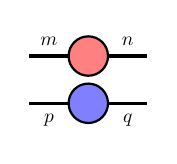
\begin{tikzpicture}[baseline=-0.5ex]
    \tikzset{tensor/.style = {minimum size = 0.5cm,shape = circle,thick,draw=black,inner sep = 0pt}, edge/.style   = {thick,line width=.4mm}}
    \def\x{0}
    \def\y{0}
    \node[tensor,fill=red!50!white] (A) at (\x,\y+0.3){$\Ab$};
    \node[tensor,fill=blue!50!white] (B) at (\x,\y-0.3){$\Bb$};
    \draw[edge] (\x-0.25,\y+0.3) -- (\x-0.75,\y+0.3) node [midway,above] {\scalebox{0.7}{\dimcolor{$m$}}};
    \draw[edge] (\x-0.25,\y-0.3) -- (\x-0.75,\y-0.3) node [midway,below] {\scalebox{0.7}{\dimcolor{$p$}}};
    \draw[edge] (\x+0.25,\y+0.3) -- (\x+0.75,\y+0.3) node [midway,above] {\scalebox{0.7}{\dimcolor{$n$}}};
    \draw[edge] (\x+0.25,\y-0.3) -- (\x+0.75,\y-0.3) node [midway,below] {\scalebox{0.7}{\dimcolor{$q$}}};
\end{tikzpicture}
\longrightarrow
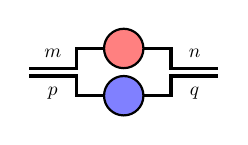
\begin{tikzpicture}[baseline=-0.5ex]
    \tikzset{tensor/.style = {minimum size = 0.5cm,shape = circle,thick,draw=black,inner sep = 0pt}, edge/.style   = {thick,line width=.4mm}}
    \def\x{0}
    \def\y{0}
    \node[tensor,fill=red!50!white] (A) at (\x,\y+0.3){$\Ab$};
    \node[tensor,fill=blue!50!white] (B) at (\x,\y-0.3){$\Bb$};
    \draw[edge] (\x-0.25,\y+0.3) -- (\x-0.6,\y+0.3) -- (\x-0.6,\y+0.05)   -- (\x-1.2,\y+0.05) node [midway,above] {\scalebox{0.7}{\dimcolor{$m$}}};
    \draw[edge] (\x-0.25,\y-0.3) -- (\x-0.6,\y-0.3) -- (\x-0.6,\y-0.05) -- (\x-1.2,\y-0.05) node [midway,below] {\scalebox{0.7}{\dimcolor{$p$}}};
    \draw[edge] (\x+0.25,\y+0.3) -- (\x+0.6,\y+0.3) -- (\x+0.6,\y+0.05) -- (\x+1.2,\y+0.05) node [midway,above] {\scalebox{0.7}{\dimcolor{$n$}}};
    \draw[edge] (\x+0.25,\y-0.3) -- (\x+0.6,\y-0.3) -- (\x+0.6,\y-0.05) -- (\x+1.2,\y-0.05) node [midway,below] {\scalebox{0.7}{\dimcolor{$q$}}};
\end{tikzpicture}
=\Ab \kron \Bb.
$$




More generally, the Kronecker product can be defined for any two tensors with the same order. It is obtained by grouping together and in order each pair of legs 
of the two tensors, e.g., 
$$
\At\kron\Bt = 
   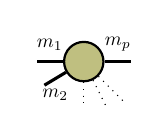
\begin{tikzpicture}[baseline=-0.5ex]
    \tikzset{tensor/.style = {minimum size = 0.5cm,shape = circle,thick,draw=black,inner sep = 0pt}, edge/.style = {thick,line width=.4mm},every loop/.style={}}
    \def\x{6}
    \node[tensor,fill=green!50!red!50!white] (A) at (\x,0) {$\At$};
    \draw[edge] (A) -- (\x-0.6,0) node [midway,above] {\scalebox{0.7}{\dimcolor{$m_1$}}};
    \draw[edge] (A) -- (\x+0.6,0) node [midway,above] {\scalebox{0.7}{\dimcolor{$m_p$}}};;
    \draw[edge] (A) -- (\x-0.5,-0.3) node [midway, below] {\scalebox{0.7}{\dimcolor{$m_2$}}};;
    \draw[dotted] (A) -- (\x,-0.6);
    \draw[dotted] (A) -- (\x,-0.6);
    \draw[dotted] (A) -- (\x+0.5,-0.5);

    \draw[dotted] (A) -- (\x+0.3,-0.6);
    \end{tikzpicture}
\kron
    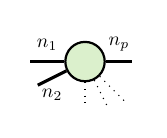
\begin{tikzpicture}[baseline=-0.5ex]
    \tikzset{tensor/.style = {minimum size = 0.5cm,shape = circle,thick,draw=black,inner sep = 0pt}, edge/.style = {thick,line width=.4mm},every loop/.style={}}
    \def\x{6}
    \def\y{0}
    \node[tensor,fill=green!70!red!20!white] (B) at (\x+1,\y) {$\Bt$};
    \draw[edge] (B) -- (\x+0.3,0) node [midway,above] {\scalebox{0.7}{\dimcolor{$n_1$}}};
    \draw[edge] (B) -- (\x+1.6,0) node [midway,above] {\scalebox{0.7}{\dimcolor{$n_p$}}};;
    \draw[edge] (B) -- (\x+0.4,-0.3) node [midway, below] {\scalebox{0.7}{\dimcolor{$n_2$}}};;
    \draw[dotted] (B) -- (\x+1,-0.6);
    \draw[dotted] (B) -- (\x+1.5,-0.5);
    \draw[dotted] (B) -- (\x+1.3,-0.6);
\end{tikzpicture}
=
    \begin{tikzpicture}[baseline=-0.5ex]
    \tikzset{tensor/.style = {minimum width = 3cm,minimum height = 0.6cm,shape = rounded rectangle,thick,draw=black,inner sep = 0pt}, edge/.style = {thick,line width=.4mm},every loop/.style={}}
    \def\x{0}
    \def\y{0}
    \node[tensor,fill=green!30!white] (At) at (\x,\y){$\At\kron\Bt$};
    \draw[edge] (\x-1.25,\y-0.3) -- (\x-1.25,\y-0.6) -- (\x-1.1,\y-0.6) -- (\x-1.1,\y-0.8);
    \draw[edge] (\x-0.85,\y-0.3) -- (\x-0.85,\y-0.6) -- (\x-1,\y-0.6) -- (\x-1,\y-0.8)node [below] {\scalebox{0.7}{\dimcolor{$m_1n_1$}}};
    \draw[edge] (\x-0.65,\y-0.3) -- (\x-0.65,\y-0.6) -- (\x-0.5,\y-0.6) -- (\x-0.5,\y-0.8);
    \draw[edge] (\x-0.25,\y-0.3) -- (\x-0.25,\y-0.6) -- (\x-0.4,\y-0.6) -- (\x-0.4,\y-0.8) node [below] {\scalebox{0.7}{\dimcolor{$m_2n_2$}}};
    \draw[edge] (\x+1.25,\y-0.3) -- (\x+1.25,\y-0.6) -- (\x+1.1,\y-0.6) -- (\x+1.1,\y-0.8);
    \draw[edge] (\x+0.85,\y-0.3) -- (\x+0.85,\y-0.6) -- (\x+1,\y-0.6) -- (\x+1,\y-0.8)  node [below] {\scalebox{0.7}{\dimcolor{$m_pn_p$}}};
    \draw[dotted] (\x+0.1,\y-0.3) -- (\x+0.1,\y-0.6) -- (\x+0.25,\y-0.6) -- (\x+0.25,\y-0.8);
    \draw[dotted] (\x+0.5,\y-0.3) -- (\x+0.5,\y-0.6) -- (\x+0.35,\y-0.6) -- (\x+0.35,\y-0.82) node [below] {\scalebox{0.7}{\dimcolor{$\dots$}}};;
    \end{tikzpicture}
    \in\RR^{m_1n_1\times\dots\times m_pn_p}.
$$

\begin{remark}
In the following, we list some useful properties of the Kronecker product.
\begin{enumerate}
    \item The Kronecker product is not commutative, i.e., $\Ab\kron\Bb \neq \Bb\kron\Ab$ in general%
    . 
    \item
    $
    \Ib\kron\Ab = 
    \begin{bmatrix}
    \Ab & 0 & \dots & 0\\
    0 & \Ab & \dots & 0\\
    \vdots & \vdots & \ddots & \vdots\\
    0 & 0 & \dots & \Ab
    \end{bmatrix}
    $
    is a block diagonal matrix.
    \item The Kronecker product of two tensors of the same order results in a tensor of the same order, while their outer product produces a tensor with double the order.
    \item 
    By reshaping the Kronecker product $\Ab\kron\Bb$, the outer product $\Ab\outprod\Bb$ can be obtained.
 \item
The Kronecker product of two {identity matrices} is a larger identity matrix, i.e., $\Ib_m \kron \Ib_n = \Ib_{mn}$, which can easily be seen by drawing the tensor network diagram: 
$$
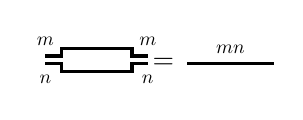
\begin{tikzpicture}[baseline=-0.5ex]
    \tikzset{tensor/.style = {minimum width = 3cm,minimum height = 0.6cm,shape = rounded rectangle,thick,draw=black,inner sep = 0pt}, edge/.style = {thick,line width=.4mm},every loop/.style={}}
    \def\x{0}
    \def\y{0.1}
    \draw[edge](\x-0.1,\y) node [above] {\scalebox{0.7}{\dimcolor{$m$}}}  -- (\x+0.1,\y) -- (\x+0.1,\y+0.1)--(\x+1,\y+0.1) -- (\x+1,\y)-- (\x+1.2,\y) node [above] {\scalebox{0.7}{\dimcolor{$m$}}};
    \draw[edge](\x-0.1,\y-0.1)  node [below] {\scalebox{0.7}{\dimcolor{$n$}}}  -- (\x+0.1,\y-0.1) -- (\x+0.1,\y-0.2)--(\x+1,\y-0.2) -- (\x+1,\y-0.1) --(\x+1.2,\y-0.1)  node [below] {\scalebox{0.7}{\dimcolor{$n$}}} ;
    \node[draw=none] at (\x+1.4,\y-0.1) {\scalebox{1}{\textcolor{black}{$=$}}};
    \draw[edge](\x+1.7,\y-0.1) -- (\x+2.8,\y-0.1) node [midway, above] {\scalebox{0.7}{\dimcolor{$mn$}}} ;
\end{tikzpicture}.
$$
     \item
     The Kronecker product of two vectors is the vectorization of their outer product: 
     $$\vectorize(\ub \outprod \vb) = \vectorize(\ub  \vb^\ts) =\ub \kron \vb =  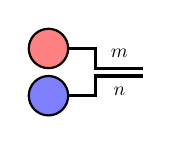
\begin{tikzpicture}[baseline=-0.5ex]
    \tikzset{tensor/.style = {minimum size = 0.5cm,shape = circle,thick,draw=black,inner sep = 0pt}, edge/.style   = {thick,line width=.4mm}}
    \def\x{0}
    \def\y{0}
    \node[tensor,fill=red!50!white] (A) at (\x,\y+0.3){$\ub$};
    \node[tensor,fill=blue!50!white] (B) at (\x,\y-0.3){$\vb$};
    \draw[edge] (\x+0.25,\y+0.3) -- (\x+0.6,\y+0.3) -- (\x+0.6,\y+0.05) -- (\x+1.2,\y+0.05) node [midway,above] {\scalebox{0.7}{\dimcolor{$m$}}};
    \draw[edge] (\x+0.25,\y-0.3) -- (\x+0.6,\y-0.3) -- (\x+0.6,\y-0.05) -- (\x+1.2,\y-0.05) node [midway,below] {\scalebox{0.7}{\dimcolor{$n$}}};
\end{tikzpicture}
    .$$
    \item 
   The Kronecker product satisfies the so-called \textit{mixed product} property: $(\Ab\kron \Bb)(\Cb\kron\Db) = \Ab\Cb\kron\Bb\Db$ where $\Ab\in\RR^{m\times n},\Bb\in\RR^{p\times q},\Cb\in\RR^{n\times d}$ and $\Db\in\RR^{q\times k}$.
\begin{proof}
 \begin{align*}
(\Ab\kron\Bb)(\Cb\kron\Db) 
&= 
\begin{tikzpicture}[baseline=\baseline]
    \tikzset{tensor/.style = {minimum size = 0.5cm,shape = circle,thick,draw=black,inner sep = 0pt}, edge/.style   = {thick,line width=.4mm}}
    \def\y{0.4}\def\x{0}
    \draw[edge] (\x-1,\y-0.3) -- (\x-0.7,\y-0.3) -- (\x-0.7,\y+0.1)   -- (\x+0.7,\y+0.1) -- (\x+0.7,\y-0.3) -- (\x+1.1,\y-0.3);
    \node[tensor,fill=red!50!white] (A) at (\x,\y){$\Ab$};
    \draw[edge] (\x+1,\y-0.3) -- (\x+1.3,\y-0.3) -- (\x+1.3,\y+0.1)   -- (\x+2.6,\y+0.1) -- (\x+2.6,\y-0.3) -- (\x+3,\y-0.3);
    \node[tensor,fill=orange!50!white] (C) at (\x+2,\y){$\Cb$};
    \def\y{-0.4}\def\x{0}
    \draw[edge] (\x-1,\y+0.4) -- (\x-0.7,\y+0.4) -- (\x-0.7,\y+0.1) -- (\x+0.7,\y+0.1) -- (\x+0.7,\y+0.4) -- (\x+0.7,\y+0.4) -- (\x+1.1,\y+0.4);
    \node[tensor,fill=blue!50!white] (B) at (\x,\y+0.1){$\Bb$};
    \draw[edge] (\x+1,\y+0.4) -- (\x+1.3,\y+0.4) -- (\x+1.3,\y+0.1) -- (\x+2.6,\y+0.1) -- (\x+2.6,\y+0.4) -- (\x+2.6,\y+0.4) -- (\x+3,\y+0.4);
    \node[draw=none] () at (\x+3.25,\y+0.45) {\scalebox{0.7}{\dimcolor{$dk$}}};
    \node[tensor,fill=green!50!red!40!white] (D) at (\x+2,\y+0.1){$\Db$};
    \node[draw=none] () at (\x+1,\y+0.7) {\scalebox{0.7}{\dimcolor{$nq$}}};
    \node[draw=none] () at (\x-1.25,\y+0.4) {\scalebox{0.7}{\dimcolor{$mp$}}};
\end{tikzpicture}\\
 &=
 \begin{tikzpicture}[baseline=\baseline]
    \tikzset{tensor/.style = {minimum size = 0.5cm,shape = circle,thick,draw=black,inner sep = 0pt}, edge/.style   = {thick,line width=.4mm}}
    \def\y{0.4}\def\x{0}
    \draw[edge] (\x-1,\y-0.35) -- (\x-0.7,\y-0.35) -- (\x-0.7,\y)   -- (\x,\y) -- (\x+0.5,\y) -- (\x+0.8,\y);
    \node[tensor,fill=red!50!white] (A) at (\x,\y){$\Ab$};
    \draw[edge] (\x+1.2,\y) -- (\x+1.7,\y) -- (\x+1.7,\y-0.35) -- (\x+2.1,\y-0.35);
    \node[tensor,fill=orange!50!white] (C) at (\x+1,\y){$\Cb$};
    \def\y{-0.4}\def\x{0}
    \draw[edge] (\x-1,\y+0.35) -- (\x-0.7,\y+0.35) -- (\x-0.7,\y) -- (\x,\y) -- (\x+0.8,\y);
    \node[tensor,fill=blue!50!white] (B) at (\x,\y){$\Bb$};
    \draw[edge] (\x+1,\y) -- (\x+1.7,\y) -- (\x+1.7,\y+0.35) -- (\x+2.1,\y+0.35);
    \node[draw=none] () at (\x+2.35,\y+0.4) {\scalebox{0.7}{\dimcolor{$dk$}}};
    \node[tensor,fill=green!50!red!40!white] (D) at (\x+1,\y){$\Db$};
    \node[draw=none] () at (\x-1.25,\y+0.35) {\scalebox{0.7}{\dimcolor{$mp$}}};
    \node[draw=none] () at (\x+0.5,\y+1) {\scalebox{0.7}{\dimcolor{$n$}}};
     \node[draw=none] () at (\x+0.5,\y+0.2) {\scalebox{0.7}{\dimcolor{$q$}}};
\end{tikzpicture}\\
&=
\Ab\Cb\kron\Bb\Db.
    \end{align*}
\end{proof}
As a special case, we have $(\Ab\kron\Ib)(\Ib\kron\Bb)=\Ab\kron\Bb$. 
\item As we can see in the derivation above, it is often useful to reshape
$
    \begin{tikzpicture}[baseline=\baseline]
    \tikzset{tensor/.style = {minimum size = 0.5cm,shape = circle,thick,draw=black,inner sep = 0pt}, edge/.style   = {thick,line width=.4mm}}
    \def\y{0.6}\def\x{0}
    \draw[edge] (\x+3,\y-0.3)  node [above] {\scalebox{0.7}{\textcolor{gray}{$p$}}} -- (\x+4,\y-0.3)node [above] {\scalebox{0.7}{\textcolor{gray}{$n$}}};
    \def\y{-0.6}\def\x{0}
    \draw[edge] (\x+3,\y+0.3) node [above] {\scalebox{0.7}{\dimcolor{$m$}}}-- (\x+4,\y+0.3)node [above] {\scalebox{0.7}{\dimcolor{$q$}}};
    \end{tikzpicture}
$
as
$
 \begin{tikzpicture}[baseline=\baseline]
    \tikzset{tensor/.style = {minimum size = 0.5cm,shape = circle,thick,draw=black,inner sep = 0pt}, edge/.style   = {thick,line width=.4mm}}
    \def\y{0.4}\def\x{0}
    \draw[edge] (\x-1,\y-0.3) -- (\x-0.7,\y-0.3)-- (\x-0.7,\y+0.1) -- (\x+0.7,\y+0.1) -- (\x+0.7,\y-0.3) -- (\x+1.1,\y-0.3);
    \node[draw=none] () at (\x+1.35,\y-0.4) {\scalebox{0.7}{\dimcolor{$nq$}}};
    \node[draw=none] () at (\x-1.25,\y-0.4) {\scalebox{0.7}{\dimcolor{$pm$}}};
    \def\y{-0.4}\def\x{0}
    \draw[edge] (\x-1,\y+0.4) -- (\x-0.7,\y+0.4) -- (\x-0.7,\y+0.1) -- (\x+0.7,\y+0.1) -- (\x+0.7,\y+0.4) -- (\x+0.7,\y+0.4) -- (\x+1.1,\y+0.4);
    \end{tikzpicture}
$ and vice versa when dealing with identities involving Kronecker products.
\item For $\Ab\in\RR^{m\times m}$ and $\Bb\in\RR^{n\times n},$ we have the equality $\tr(\Ab\kron\Bb)=\tr(\Ab)\tr(\Bb)$, which can easily be proved by the following diagram:
$$
\tr(\Ab\kron\Bb) = 
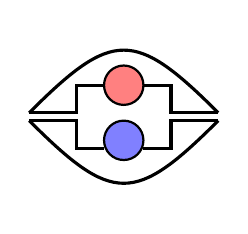
\begin{tikzpicture}[baseline=-0.5ex]
    \tikzset{tensor/.style = {minimum size = 0.5cm,shape = circle,thick,draw=black,inner sep = 0pt}, edge/.style   = {thick,line width=.4mm}}
    \def\x{0}
    \def\y{0}
    \node[tensor,fill=red!50!white] (A) at (\x,\y+0.5){$\Ab$};
    \node[tensor,fill=blue!50!white] (B) at (\x,\y-0.2){$\Bb$};
    \draw[edge] (\x-0.25,\y+0.5) -- (\x-0.6,\y+0.5) -- (\x-0.6,\y+0.15)   -- (\x-1.2,\y+0.15);
    \draw[edge] (\x-0.25,\y-0.3) -- (\x-0.6,\y-0.3) -- (\x-0.6,\y+0.05) -- (\x-1.2,\y+0.05);
    \draw[edge] (\x+0.25,\y+0.5) -- (\x+0.6,\y+0.5) -- (\x+0.6,\y+0.15) -- (\x+1.2,\y+0.15);
    \draw[edge] (\x+0.25,\y-0.3) -- (\x+0.6,\y-0.3) -- (\x+0.6,\y+0.05) -- (\x+1.2,\y+0.05);
    \draw[edge](\x-1.2,\y+0.15) to [out=45,in=135, distance=1.5cm] (\x+1.2,\y+0.15);
    \draw[edge](\x-1.2,\y+0.05) to [out=-45,in=-135, distance=1.5cm] (\x+1.2,\y+0.05);
\end{tikzpicture}
=
\tr(\Ab)\tr(\Bb).
$$

\item The \textbf{Sylvester Identity} is a very useful identity connecting vectorization, matrix product, and Kronecker product: $$\vectorize(\Ab\Xb\Bb) = (\Ab\kron \Bb^\ts)\vectorize(\Xb),$$
where $\Ab\in\RR^{m\times n},\Xb\in\RR^{n\times p}$ and $\Bb\in\RR^{p\times q}.$
\begin{proof}
The proof is rather direct using tensor networks: 
\begin{align*}
\vectorize(\Ab\Xb\Bb) &=
 \vectorize\left(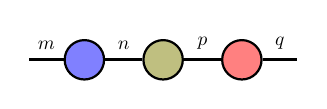
\begin{tikzpicture}[baseline=-0.5ex]
    \tikzset{tensor/.style = {minimum size = 0.5cm,shape = circle,thick,draw=black,inner sep = 0pt}, edge/.style = {thick,line width=.4mm},every loop/.style={}}
    \def\x{6}
    \node[tensor,fill=blue!50!white] (A) at (\x-1,0) {$\Ab$};
    \node[tensor,fill=green!50!red!50!white] (X) at (\x,0) {$\Xb$};
    \node[tensor,fill=red!50!white] (B) at (\x+1,0) {$\Bb$};
    \draw[edge] (A) -- (X) node [midway,above] {\scalebox{0.7}{\dimcolor{$n$}}};
    \draw[edge] (X) -- (B) node [midway,above] {\scalebox{0.7}{\dimcolor{$p$}}};
    \draw[edge] (A) -- (\x-1.7,0) node [midway,above] {\scalebox{0.7}{\dimcolor{$m$}}};
    \draw[edge] (B) -- (\x+1.7,0) node [midway,above] {\scalebox{0.7}{\dimcolor{$q$}}};
    \end{tikzpicture}\right)
=
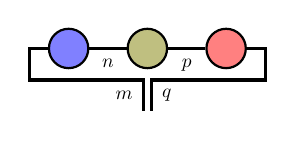
\begin{tikzpicture}[baseline=-0.5ex]
    \tikzset{tensor/.style = {minimum size = 0.5cm,shape = circle,thick,draw=black,inner sep = 0pt}, edge/.style = {thick,line width=.4mm},every loop/.style={}}
    \def\x{6}
    \node[tensor,fill=blue!50!white] (A) at (\x-1,0) {$\Ab$};
    \node[tensor,fill=green!50!red!50!white] (X) at (\x,0) {$\Xb$};
    \node[tensor,fill=red!50!white] (B) at (\x+1,0) {$\Bb$};
    \draw[edge] (A) -- (X) node [midway,below] {\scalebox{0.7}{\dimcolor{$n$}}};
    \draw[edge] (X) -- (B) node [midway,below] {\scalebox{0.7}{\dimcolor{$p$}}};
    \draw[edge] (A) -- (\x-1.5,0) -- (\x-1.5,-0.4) -- (\x-0.05,-0.4)--(\x-0.05,-0.8) node [midway,left] {\scalebox{0.7}{\dimcolor{$m$}}};
    \draw[edge] (B) -- (\x+1.5,0) -- (\x+1.5,-0.4) -- (\x+0.05,-0.4)--(\x+0.05,-0.8) node [midway,right] {\scalebox{0.7}{\dimcolor{$q$}}};
\end{tikzpicture}\\
&=
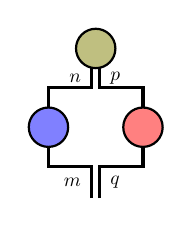
\begin{tikzpicture}[baseline=-2ex]
    \tikzset{tensor/.style = {minimum size = 0.5cm,shape = circle,thick,draw=black,inner sep = 0pt}, edge/.style = {thick,line width=.4mm},every loop/.style={}}
    \def\x{6}
    \draw[edge] (\x-0.05,0.25) -- (\x-0.05,0) node [midway, left] {\scalebox{0.7}{\dimcolor{$n$}}}   -- (\x-0.6,0) -- (\x-0.6,-0.25) ; 
    \draw[edge] (\x+0.05,0.25) -- (\x+0.05,0)   node [midway, right] {\scalebox{0.7}{\dimcolor{$p$}}}  -- (\x+0.6,0) -- (\x+0.6,-0.25);    
    \draw[edge] (\x-0.05,-1.4) -- (\x-0.05,-1)  node [midway, left] {\scalebox{0.7}{\dimcolor{$m$}}}  -- (\x-0.6,-1) -- (\x-0.6,-0.75) ; 
    \draw[edge] (\x+0.05,-1.4) -- (\x+0.05,-1)  node [midway, right] {\scalebox{0.7}{\dimcolor{$q$}}}   -- (\x+0.6,-1) -- (\x+0.6,-0.75); 
     \node[tensor,fill=green!50!red!50!white] (X) at (\x,0.5) {$\Xb$};
    \node[tensor,fill=blue!50!white] (A) at (\x-0.6,-0.5) {$\Ab$};
    \node[tensor,fill=red!50!white] (B) at (\x+0.6,-0.5) {$\Bb$};
\end{tikzpicture}
=
(\Ab\kron\Bb^\ts)\vectorize(\Xb).
\end{align*}
It is easy in the last diagram to identify the vectorization of $\Xb$ and the Kronecker product of $\Ab$ and $\Bb$, and thus to conclude that this tensor network represents a matrix-vector product between the two. However, when translating the tensor network in classical mathematical notation, some care is required. First, we can see that since $\vectorize(\Xb)$ is of dimension $np$, the Kronecker product has to be between $\Ab$ and $\Bb^\ts$ to obtain a matrix of shape $mq\times np$. Then, we need to know which Kronecker product to use: $\Ab \kron \Bb^\ts$ or $\Bb^\ts \kron \Ab$, which are both of the correct shape. Because in this manuscript we use lexicographic ordering for reshape operations such as $\vectorize$, the correct formulation is  $\Ab \kron \Bb^\ts$. However, if we were to use reverse lexicographic ordering, as in~\citep{kolda2009tensor}, the correct formulation would be $\Bb^\ts \kron \Ab$.
\end{proof}
The \emph{Sylvester identity} is a useful identity to solve  systems of equations of the form $\Ab\Xb+\Xb\Bb = \Cb$.
\end{enumerate}
\end{remark}
There are useful relationships between the $n$-mode product, matricization, and Kronecker products: 
\begin{proposition}
Let $\Tt\in\RR^{d_1\times d_2\times\dots\times d_p}$, $\Ab_1\in\RR^{d_1\times n_1},
\Ab_2\in\RR^{d_2\times n_2},\dots,$
$\Ab_p\in\RR^{d_p\times n_p}$, then 
\begin{align*}(\Tt\ttm1\Ab_1\ttm2\Ab_2\ttm3\Ab_3\ttm4\dots\ttm p\Ab_p)_{(n)}=
\Ab_n\Tt_{(n)}(\Ab_1\kron\dots\kron\Ab_{n-1}\kron\Ab_{n+1}\kron\dots\kron\Ab_p)^\ts.
\end{align*}
\end{proposition}
\begin{proof}
For $p =3$ and $n=1$,
\begin{align*}
(\Tt\ttm1\Ab_1\ttm2\Ab_2\ttm3\Ab_3)_{(1)}
&= 
 \left(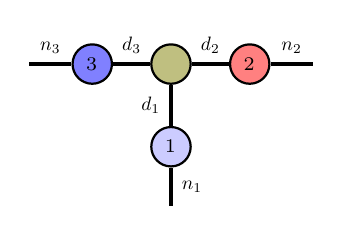
\begin{tikzpicture}[baseline=-0.5ex]
    \tikzset{tensor/.style = {minimum size = 0.5cm,shape = circle,thick,draw=black,inner sep = 0pt}, edge/.style = {thick,line width=.4mm},every loop/.style={}}
    \def\x{6}
    \node[tensor,fill=blue!20!white] (A1) at (\x,-1.05) {$\Ab_1$};
    \node[tensor,fill=green!50!red!50!white] (At) at (\x,0) {$\Tt$};
    \node[tensor,fill=red!50!white] (A2) at (\x+1,0) {$\Ab_2$};
    \node[tensor,fill=blue!50!white] (A3) at (\x-1,0) {$\Ab_3$};
    \draw[edge] (At) -- (A2) node [midway,above] {\scalebox{0.7}{\dimcolor{$d_2$}}};
    \draw[edge] (At) -- (A1) node [midway,left] {\scalebox{0.7}{\dimcolor{$d_1$}}};
    \draw[edge] (At) -- (A3) node [midway,above] {\scalebox{0.7}{\dimcolor{$d_3$}}};
    \draw[edge] (A1) -- (\x,-1.8) node [midway,right] {\scalebox{0.7}{\dimcolor{$n_1$}}};
    \draw[edge] (A2) -- (\x+1.8,0) node [midway,above] {\scalebox{0.7}{\dimcolor{$n_2$}}};
    \draw[edge] (A3) -- (\x-1.8,0) node [midway,above] {\scalebox{0.7}{\dimcolor{$n_3$}}};
    \end{tikzpicture}\right)_{(1)}
=
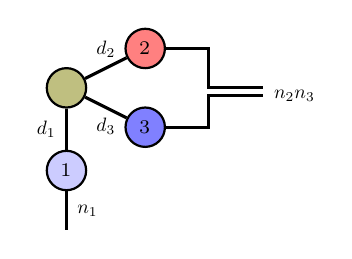
\begin{tikzpicture}[baseline=-0.5ex]
    \tikzset{tensor/.style = {minimum size = 0.5cm,shape = circle,thick,draw=black,inner sep = 0pt}, edge/.style = {thick,line width=.4mm},every loop/.style={}}
    \def\x{6}
    \def\y{0}
    \node[tensor,fill=blue!20!white] (A1) at (\x,-1.05) {$\Ab_1$};
    \node[tensor,fill=green!50!red!50!white] (At) at (\x,0) {$\Tt$};
    \node[tensor,fill=red!50!white] (A2) at (\x+1,\y+0.5) {$\Ab_2$};
    \node[tensor,fill=blue!50!white] (A3) at (\x+1,\y-0.5) {$\Ab_3$};
    \draw[edge] (At) -- (A1) node [midway,left] {\scalebox{0.7}{\dimcolor{$d_1$}}};
    \draw[edge] (At) -- (A3) node [midway,below] {\scalebox{0.7}{\dimcolor{$d_3$}}};
    \draw[edge] (At) -- (A2) node [midway,above] {\scalebox{0.7}{\dimcolor{$d_2$}}};
    \draw[edge] (A1) -- (\x,-1.8) node [midway,right] {\scalebox{0.7}{\dimcolor{$n_1$}}};
    \draw[edge] (A2) -- (\x+1.8,\y+0.5) -- (\x+1.8,\y)-- (\x+2.5,\y);
    \draw[edge] (A3) -- (\x+1.8,\y-0.5) -- (\x+1.8,\y-0.1) -- (\x+2.5,\y-0.1)node [right] {\scalebox{0.7}{\dimcolor{$n_2n_3$}}};
    \end{tikzpicture}\\
&=
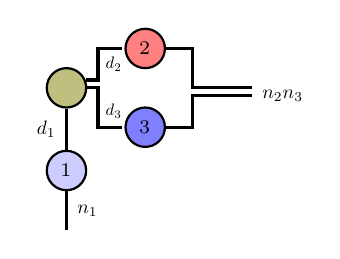
\begin{tikzpicture}[baseline=-0.5ex]
    \tikzset{tensor/.style = {minimum size = 0.5cm,shape = circle,thick,draw=black,inner sep = 0pt}, edge/.style = {thick,line width=.4mm},every loop/.style={}}
    \def\x{6}
    \def\y{0}
    \node[tensor,fill=blue!20!white] (A1) at (\x,-1.05) {$\Ab_1$};
    \node[tensor,fill=green!50!red!50!white] (At) at (\x,0) {$\Tt$};
    \node[tensor,fill=red!50!white] (A2) at (\x+1,\y+0.5) {$\Ab_2$};
    \node[tensor,fill=blue!50!white] (A3) at (\x+1,\y-0.5) {$\Ab_3$};
    \draw[edge] (At) -- (A1) node [midway,left] {\scalebox{0.7}{\dimcolor{$d_1$}}};
    \draw[edge] (\x+0.7,\y-0.5) -- (\x+0.4,\y-0.5) -- (\x+0.4,\y) -- (\x+0.25,\y);
    \draw[edge] (\x+0.7,\y+0.5) -- (\x+0.4,\y+0.5) -- (\x+0.4,\y+0.1) -- (\x+0.25,\y+0.1);
    \draw[edge] (A1) -- (\x,-1.8) node [midway,right] {\scalebox{0.7}{\dimcolor{$n_1$}}};
    \draw[edge] (A2) -- (\x+1.6,\y+0.5) -- (\x+1.6,\y)-- (\x+2.35,\y);
    \draw[edge] (A3) -- (\x+1.6,\y-0.5) -- (\x+1.6,\y-0.1) -- (\x+2.35,\y-0.1)node [right] {\scalebox{0.7}{\dimcolor{$n_2n_3$}}};
    \node[draw=none] () at (\x+0.6,\y-0.3) {\scalebox{0.6}{\dimcolor{$d_3$}}};
    \node[draw=none] () at (\x+0.6,\y+0.3) {\scalebox{0.6}{\dimcolor{$d_2$}}};
\end{tikzpicture}
=
\Ab_1\Tt_{(1)}(\Ab_2\kron\Ab_3)^\ts.
\end{align*}
\end{proof}
\begin{proposition}
    Let $\Tt\in\RR^{d_1\times d_2\times\cdots\times d_p}$  and $\Ab_i\in\RR^{d_i\times n_i}$ for $i\in[p]$. Let $m \in [p]$ and
$\Tt_{([m])}$ denotes reshaping the tensor $\Tt$ in a matrix of size $d_1d_2\cdots d_m\times d_{m+1}...d_p$ by mapping the first $m$ indices to
rows and the remaining ones to columns. Then,
\begin{align*}
    (\Tt\ttm 1\Ab_1\ttm 2 \Ab_2\cdots\ttm p \Ab_p)_{([m])}=(\Ab_1\kron\Ab_2\kron\cdots\kron\Ab_{m})\Tb_{([m])}(\Ab_{m+1}\kron\Ab_{m+2}\kron\cdots\kron\Ab_{p})^\ts.
\end{align*}
This identity can be extended to arbitrary subsets $I\subset [p]$:
$$ (\Tt\ttm 1\Ab_1\ttm 2 \Ab_2\cdots\ttm p \Ab_p)_{(I)}    = \left(\bigotimes_{i\in I} \Ab_i\right)\Tt_{([m])}\left(\bigotimes_{i\in [p] \setminus I} \Ab_i\right)^\ts.$$
\begin{proof}
For $p=6$ and $I = \{1,2,3\}$,
\begin{align*}
\left(\begin{tikzpicture}[baseline=\baseline]
    \tikzset{tensor/.style = {minimum size = 0.5cm,shape = circle,thick,draw=black,inner sep = 0pt}, edge/.style = {thick,line width=.4mm},every loop/.style={}}
    \def\y{0}
    \def\x{0}
    \node[tensor,fill=red!20!blue!40!white] (T) at (\x,\y){\scalebox{0.85}{$\Tt$}};
\node[tensor,fill=red!20!white] (A) at (\x+1,\y){\scalebox{0.85}{$\Ab_1$}};
    \draw[edge](T) -- (A) node [midway,above] {\scalebox{0.7}{\dimcolor{$d_1$}}};
    \draw[edge](A) -- (\x+2,\y) node [midway,above] {\scalebox{0.7}{\dimcolor{$n_1$}}};
\node[tensor,fill=red!40!white] (B) at (\x,\y-1) {\scalebox{0.85}{$\Ab_2$}}; 
    \draw[edge](T) -- (B) node [midway,left] {\scalebox{0.7}{\dimcolor{$d_2$}}};
    \draw[edge](B) -- (\x,\y-2) node [midway,left] {\scalebox{0.7}{\dimcolor{$n_2$}}};
\node[tensor,fill=red!60!white] (C) at (\x-1,\y) {\scalebox{0.85}{$\Ab_3$}};
    \draw[edge](T) -- (C) node [midway,above] {\scalebox{0.7}{\dimcolor{$d_3$}}};
    \draw[edge](C) -- (\x-2,\y) node [midway,above] {\scalebox{0.7}{\dimcolor{$n_3$}}};
\node[tensor,fill=blue!20!white] (D) at (\x,\y+1){\scalebox{0.85}{$\Ab_4$}}; 
    \draw[edge](T) -- (D) node [midway,right] {\scalebox{0.7}{\dimcolor{$d_4$}}};
    \draw[edge](D) -- (\x,\y+2) node [midway,right] {\scalebox{0.7}{\dimcolor{$n_4$}}};
\node[tensor,fill=red!50!blue!10!white] (E) at (\x-0.85,\y+0.85){\scalebox{0.85}{$\Ab_5$}}; 
   \draw[edge](T) -- (E) node [midway,above] {\scalebox{0.7}{\dimcolor{$d_5$}}};
    \draw[edge](E) -- (\x-1.5,\y+1.5) node [midway,right] {\scalebox{0.7}{\dimcolor{$n_5$}}};
\node[tensor,fill=blue!50!white] (F) at (\x+0.85,\y-0.85){\scalebox{0.85}{$\Ab_6$}};
    \draw[edge](T) -- (F)node [midway,right] {\scalebox{0.7}{\dimcolor{$d_6$}}};
    \draw[edge](F) -- (\x+1.5,\y-1.5)node [midway,right] {\scalebox{0.7}{\dimcolor{$n_6$}}};
\end{tikzpicture}\right)_{(\{1,2,3\})}
\begin{tikzpicture}[baseline=\baseline]
    \tikzset{tensor/.style = {minimum size = 0.5cm,shape = circle,thick,draw=black,inner sep = 0pt}, edge/.style = {thick,line width=.4mm},every loop/.style={}}
    \def\y{0}
    \def\x{0}
    \node[draw=none] at (\x-3.5,\y){$=$};
    \node[tensor,fill=red!20!blue!40!white] (T) at (\x,\y){\scalebox{0.85}{$\Tb$}};
    \node[tensor,fill=red!20!white] (A) at (\x-1.5,\y-1){\scalebox{0.85}{$\Ab_1$}};
    \node[tensor,fill=red!40!white] (B) at (\x-1.5,\y) {\scalebox{0.85}{$\Ab_2$}}; 
    \node[tensor,fill=red!60!white] (C) at (\x-1.5,\y+1) {\scalebox{0.85}{$\Ab_3$}};
    \node[tensor,fill=blue!20!white] (D) at (\x+1.5,\y-1){\scalebox{0.85}{$\Ab_4$}};
\node[tensor,fill=red!50!blue!10!white] (E) at (\x+1.5,\y){\scalebox{0.85}{$\Ab_5$}}; 
\node[tensor,fill=blue!50!white] (F) at (\x+1.5,\y+1){\scalebox{0.85}{$\Ab_6$}};
    \draw[edge](T) -- (B);
    \node[draw=none] at (\x-1.15,\y+0.2) {\scalebox{0.7}{\dimcolor{$d_2$}}};;
    \node[draw=none] at (\x+1.15,\y+0.2) {\scalebox{0.7}{\dimcolor{$d_5$}}};;
    \draw[edge](B) -- (\x-2.5,\y);;
    \draw[edge](\x+0.16,\y+0.2) -- (\x+0.5,\y+0.2) -- (\x+0.5,\y+0.1) -- (\x+1,\y+0.1);
    \draw[edge](F) -- (\x+1,\y+1) -- (\x+1,\y+0.1)node [midway,left] {\scalebox{0.7}{\dimcolor{$d_6$}}};
    \draw[edge](F) -- (\x+2,\y+1)--(\x+2,\y+0.1)-- (\x+2.5,\y+0.1)node [near end,above] {\scalebox{0.7}{\dimcolor{$n_6$}}};
    \draw[edge](\x+0.16,\y-0.2) -- (\x+0.5,\y-0.2) -- (\x+0.5,\y-0.1) -- (\x+1,\y-0.1);
    \draw[edge](D) -- (\x+1,\y-1) -- (\x+1,\y-0.1)node [midway,left] {\scalebox{0.7}{\dimcolor{$d_4$}}};
    \draw[edge](D) -- (\x+2,\y-1)--(\x+2,\y-0.1)-- (\x+2.5,\y-0.1)node [near end,below] {\scalebox{0.7}{\dimcolor{$n_4$}}};
    \draw[edge](T) -- (E);
    \draw[edge](E) -- (\x+2.5,\y);
    \draw[edge](\x-0.16,\y+0.2) -- (\x-0.5,\y+0.2) -- (\x-0.5,\y+0.1) -- (\x-1,\y+0.1);
    \draw[edge](C) -- (\x-1,\y+1) -- (\x-1,\y+0.1)node [midway,right] {\scalebox{0.7}{\dimcolor{$d_3$}}};
    \draw[edge](C) -- (\x-2,\y+1)--(\x-2,\y+0.1)-- (\x-2.5,\y+0.1)node [near end,above] {\scalebox{0.7}{\dimcolor{$n_3$}}};;;
    \draw[edge](\x-0.16,\y-0.2) -- (\x-0.5,\y-0.2) -- (\x-0.5,\y-0.1) -- (\x-1,\y-0.1);
    \draw[edge](A) --  (\x-2,\y-1)--(\x-2,\y-0.1)-- (\x-2.5,\y-0.1)node [near end,below] {\scalebox{0.7}{\dimcolor{$n_1$}}};;
    \draw[edge](A) -- (\x-1,\y-1) -- (\x-1,\y-0.1)node [midway,right] {\scalebox{0.7}{\dimcolor{$d_1$}}};
    \node[draw=none] at (\x+2.8,\y){\scalebox{0.7}{\dimcolor{$n_4$}}};
    \node[draw=none] at (\x-2.8,\y){\scalebox{0.7}{\dimcolor{$n_2$}}};
\end{tikzpicture}.
\end{align*}
\end{proof}
\end{proposition}


\paragraph{Khatri-Rao product}
The Khatri-Rao product is the column-wise Kronecker product~\citep{smilde2005multi,bro1998multi}. Let $\Ab\in\RR^{m\times R}$ and $\Bb\in\RR^{n\times R}$. The Khatri-Rao product of $\Ab$ and $\Bb$, denoted as $\Ab\krao\Bb\in\RR^{mn\times R}$, is defined by
\begin{align*}
    \def\baseline{-0.5ex}
    \Ab\krao\Bb =
    \begin{bmatrix}
    \vline & \vline  &   & \vline \\
    \ab_1\kron\bb_1 & \ab_2\kron\bb_2 & \dots & \ab_R\kron\bb_R\\
    \vline & \vline & & \vline 
    \end{bmatrix}
=
    \begin{tikzpicture}[baseline=\baseline]
    \tikzset{tensor/.style = {minimum size = 0.5cm,shape = circle,thick,draw=black,inner sep = 0pt}, edge/.style   = {thick,line width=.4mm},every loop/.style={}}
    \def\y{0}
    \def\x{0}
    \node[tensor,fill=red!50!white] (A) at (\x,\y){$\Ab$};
    \node[tensor,fill=blue!50!white] (B) at (\x+1,\y){$\Bb$};
    \draw[edge] (\x,\y+0.25) -- (\x,\y+0.5) -- (\x+0.5,\y+0.7);
    \draw[edge] (\x+1,\y+0.25) -- (\x+1,\y+0.5) -- (\x+0.5,\y+0.7);
    \draw[edge] (\x+0.5,\y+0.7) -- (\x+0.5,\y+1.2) node [left, midway] {\edgelabel{$R$}};
    \draw  node[fill = black,circle,inner sep=0pt,minimum size=4pt] (m) at (\x+0.5,\y+0.7) {};
    \draw[edge] (\x,\y-0.25) -- (\x,\y-0.7);
    \draw[edge] (\x+1,\y-0.25) -- (\x+1,\y-0.7);
    \draw[edge] (\x+1,\y-0.7) -- (\x+0.5,\y-0.7) -- (\x+0.5,\y-1);
    \draw[edge] (\x+1,\y-0.25) -- (\x+1,\y-0.7);
    \draw[edge] (\x,\y-0.7) -- (\x+0.4,\y-0.7) -- (\x+0.4,\y-1)node [below] {\edgelabel{$mn$}};
    \end{tikzpicture}\hspace{0.5cm},
\end{align*}
where $\ab_1,\dots,\ab_R\in\RR^{m}$ are the columns of $\Ab$ and $\bb_1,\dots,\bb_R\in\RR^{n}$ are the columns of $\Bb$.  In the corresponding tensor network diagram, the copy tensor enforces that the resulting matrix only contains the Kronecker product of \emph{matching} columns of $\Ab$ and $\Bb$. 
\begin{remark}
Some of the Khatri-Rao product properties are listed below:
\begin{enumerate}
\item Like the Kronecker product, the Khatri-Rao product is not commutative, i.e., $\Ab\krao\Bb\neq \Bb\krao\Ab$ in general.
\item The Khatri-Rao product is associative, i.e., $\Ab\krao(\Bb\krao\Cb)=(\Ab\krao\Bb)\krao\Cb$, where $\Ab\in\RR^{m\times R},\Bb\in\RR^{n\times R}$ and $\Cb\in\RR^{s\times R}$.
\item The columns of $\Ab\krao\Bb$ form a subset of the columns of the Kronecker product $\Ab\kron \Bb$.
\end{enumerate}
\end{remark}

\paragraph{Hadamard product}
Let $\Ab\in\RR^{m\times n}$ and $\Bb\in\RR^{m\times n}$ be matrices of the same shape. The Hadamard (or component-wise) product of $\Ab$ and $\Bb$ is the matrix  $\Ab\hadam\Bb\in\RR^{m\times n}$ defined element-wise by 
$$(\Ab\hadam\Bb)_{ij} = \Ab_{ij}\Bb_{ij}.$$
In tensor network diagrams, the Hadamard product can easily be represented using copy tensors:
\begin{equation*}
\Ab\hadam\Bb =
     \begin{tikzpicture}[baseline=\baseline]
    \tikzset{tensor/.style = {minimum size = 0.5cm,shape = circle,thick,draw=black,inner sep = 0pt}, edge/.style   = {thick,line width=.4mm},every loop/.style={}}
    \def\y{0}
    \def\x{0}
    \draw[edge] (\x,\y-0.7) -- (\x,\y+0.7)  node [very near end,left] {\edgelabel{$m$}} node [very near start,left] {\edgelabel{$n$}} ;
    \node[tensor,fill=red!50!white] (A) at (\x,\y){$\Ab$};
    \end{tikzpicture} 
    \ \hadam %
    \begin{tikzpicture}[baseline=\baseline]
    \tikzset{tensor/.style = {minimum size = 0.5cm,shape = circle,thick,draw=black,inner sep = 0pt}, edge/.style   = {thick,line width=.4mm},every loop/.style={}}
    \def\y{0}
    \def\x{0}
    \draw[edge] (\x,\y-0.7) -- (\x,\y+0.7)node [very near end,left] {\edgelabel{$m$}} node [very near start,left] {\edgelabel{$n$}} ;
    \node[tensor,fill=blue!50!white] (B) at (\x,\y){$\Bb$};
    \end{tikzpicture}
\ =
\begin{tikzpicture}[baseline=\baseline]
    \tikzset{tensor/.style = {minimum size = 0.5cm,shape = circle,thick,draw=black,inner sep = 0pt}, edge/.style   = {thick,line width=.4mm},every loop/.style={}}
    \def\y{0}
    \def\x{0}
    \node[tensor,fill=red!50!white] (A) at (\x,\y){$\Ab$};
    \node[tensor,fill=blue!50!white] (B) at (\x+1,\y){$\Bb$};
    \draw[edge] (\x,\y+0.25) -- (\x,\y+0.5) -- (\x+0.5,\y+0.7);
    \draw[edge] (\x+1,\y+0.25) -- (\x+1,\y+0.5) -- (\x+0.5,\y+0.7);
    \draw[edge] (\x+0.5,\y+0.7) -- (\x+0.5,\y+1) node [near start,left] {\edgelabel{$m$}};
    \draw  node[fill = black,circle,inner sep=0pt,minimum size=4pt] (m) at (\x+0.5,\y+0.7) {};
    \draw[edge] (\x,\y-0.25) -- (\x,\y-0.5) -- (\x+0.5,\y-0.7);
    \draw[edge] (\x+1,\y-0.25) -- (\x+1,\y-0.5) -- (\x+0.5,\y-0.7);
    \draw[edge] (\x+0.5,\y-0.7) -- (\x+0.5,\y-1) node [near start,left] {\edgelabel{$n$}};
    \draw  node[fill = black,circle,inner sep=0pt,minimum size=4pt] (m) at (\x+0.5,\y-0.7) {};
\end{tikzpicture}.
\end{equation*}
More generally, for any $\Ab_1\in\RR^{m\times n},\dots,\Ab_d\in\RR^{m\times n}$ we have 
\begin{align*}
\Ab_1\hadam\Ab_2\dots\hadam\Ab_{d} 
=
    \begin{tikzpicture}[baseline=\baseline]
    \tikzset{tensor/.style = {minimum size = 0.5cm,shape = circle,thick,draw=black,inner sep = 0pt}, edge/.style   = {thick,line width=.4mm},every loop/.style={}}
    \def\y{1}
    \def\x{0}
    \node[tensor,fill=red!30!white] (A_1) at (\x,\y){$\Ab_1$};
    \node[tensor,fill=red!30!white] (A_2) at (\x,\y-1){$\Ab_2$};
    \node[draw=none] at (\x,\y-1.5) {\scalebox{1}{\textcolor{black}{$\vdots$}}};
    \node[tensor,fill=red!30!white] (A_N) at (\x,\y-2.5){$\Ab_d$};
    \draw  node[fill = black,circle,inner sep=0pt,minimum size=4pt] (m) at (\x+1,\y-1) {};
    \draw  node[fill = black,circle,inner sep=0pt,minimum size=4pt] (n) at (\x-1,\y-1) {};
    \draw[edge] (A_1) -- (m);
    \draw[edge] (A_2) -- (m);
    \draw[edge] (A_N) -- (m);
    \draw[edge] (A_1) -- (n);
    \draw[edge] (A_2) -- (n);
    \draw[edge] (A_N) -- (n);
    \draw[edge] (m) -- (\x+1.5,\y-1)node [midway,above] {\edgelabel{$n$}};
    \draw[edge] (n) -- (\x-1.5,\y-1)node [midway,above] {\edgelabel{$m$}};
    \end{tikzpicture}.
\end{align*}
\begin{remark}
We list here some useful properties of the Hadamard product.
\begin{itemize}
    \item The Hadamard product of a tensor $\Tt$ with entries in $\{0,1\}$ with itself is $\Tt$. This is in particular true for the copy tensor:
    
    Let $\Tt\in\RR^{d_1\times d_2\times d_3}$ be a 3rd way copy tensor. Then the Hadamard product $\Tt\hadam\Tt$ in tensor networks is:
    $$\Tt\hadam\Tt=
    \begin{tikzpicture}[baseline=\baseline]
   \tikzset{tensor/.style = {minimum size = 0.5cm,shape = circle,thick,draw=black,inner sep = 0pt}, edge/.style = {thick,line width=.4mm},every loop/.style={}}
    \def\y{0.2}
    \def\x{0}
     \draw  node[fill = black,circle,inner sep=0pt,minimum size=4pt] (m) at (\x,\y-0.5) {};
     \draw  node[draw=none] (a) at (\x-0.7,\y-0.5) {};
     \draw  node[draw=none] (b) at (\x+0.7,\y-0.5) {};
     \draw  node[draw=none] (c) at (\x,\y-1.25) {};
    \draw[edge] (a) -- (m) node [midway,above] {\scalebox{0.7}{\dimcolor{$d_1$}}};
    \draw[edge] (m) -- (b)node [midway,above] {\scalebox{0.7}{\dimcolor{$d_2$}}};
    \draw[edge] (m) -- (c)node [midway,left] {\scalebox{0.7}{\dimcolor{$d_3$}}};
    \draw  node[fill = black,circle,inner sep=0pt,minimum size=4pt] (m1) at (\x,\y+0.3) {};
     \draw  node[draw=none] (d) at (\x-0.7,\y+0.3) {};
     \draw  node[draw=none] (e) at (\x+0.7,\y+0.3) {};
     \draw  node[draw=none] (f) at (\x,\y+1.05) {};
    \draw[edge] (d) -- (m1)node [midway,below] {\scalebox{0.7}{\dimcolor{$d_1$}}};
    \draw[edge] (m1) -- (e)node [midway,below] {\scalebox{0.7}{\dimcolor{$d_2$}}};
    \draw[edge] (m1) -- (f)node [midway,left] {\scalebox{0.7}{\dimcolor{$d_3$}}};
    \node[draw=none] at (\x,\y-0.15){$\hadam$};
\end{tikzpicture}
=
    \begin{tikzpicture}[baseline=\baseline]
   \tikzset{tensor/.style = {minimum size = 0.5cm,shape = circle,thick,draw=black,inner sep = 0pt}, edge/.style = {thick,line width=.4mm},every loop/.style={}}
    \def\y{0}
    \def\x{0}
    \draw[edge](\x-0.7,\y-0.5)--(\x+0.7,\y-0.5);
    \draw[edge](\x-0.7,\y+0.5)--(\x+0.7,\y+0.5);
    \draw[edge](\x-0.7,\y-0.5)--(\x-0.7,\y+0.5);
    \draw[edge](\x+0.7,\y-0.5)--(\x+0.7,\y+0.5);
    \draw[edge](\x,\y+0.5) -- (\x,\y-0.5);
     \draw  node[fill = black,circle,inner sep=0pt,minimum size=4pt] (m1) at (\x-0.7,\y) {};
    \draw  node[fill = black,circle,inner sep=0pt,minimum size=4pt] (m) at (\x,\y) {};
    \draw  node[fill = black,circle,inner sep=0pt,minimum size=4pt] (m2) at (\x+0.7,\y) {};
    \draw[edge](m1)--(\x-1,\y)node [midway,above] {\scalebox{0.7}{\dimcolor{$d_1$}}};
    \draw[edge](m2)--(\x+0.4,\y)node [midway,above] {\scalebox{0.7}{\dimcolor{$d_3$}}};
    \draw[edge](m)--(\x-0.3,\y)node [midway,above] {\scalebox{0.7}{\dimcolor{$d_2$}}};
     \end{tikzpicture}$$
    
    \item Using Proposition~\ref{prop:copy.tensor}~(items 4 and 5), we can see that 
    $\vb\hadam\ub=$
         \begin{tikzpicture}[baseline=\baseline]
    \tikzset{tensor/.style = {minimum size = 0.5cm,shape = circle,thick,draw=black,inner sep = 0pt}, edge/.style   = {thick,line width=.4mm},every loop/.style={}}
    \def\y{0}
    \def\x{0}
    \draw  node[fill = black,circle,inner sep=0pt,minimum size=4pt] (m) at (\x+0.5,\y+0.5) {};
    \node[tensor,fill=blue!20!red!40!white] (v) at (\x,\y-0.65){\scalebox{0.85}{$\vb$}};
    \node[tensor,fill=red!20!blue!40!white] (u) at (\x+1,\y-0.65){\scalebox{0.85}{$\ub$}};

    \draw[edge] (m) -- (\x,\y) -- (v); 
    
    \draw[edge] (m) -- (\x+1,\y) -- (u); 
    \draw[edge](m) -- (\x+0.5,\y+1);
    \end{tikzpicture}
    $=\text{diag}(\vb)\ub$
\end{itemize}
\end{remark}
To conclude this chapter, we introduce several useful results in the next section.

\subsection{Some Useful Properties of Tensor Networks}\label{sec:useful-TNs}
In this section, we list several useful results about tensor networks. 

\paragraph{Bounding the Rank of Matricizations.}
Any tensor network structure induces a collection of upper bounds on the matricizations of the underlying tensor. More precisely, for an arbitrary tensor network, the rank of a given matricization is bounded by the weight of any cut separating the row legs from the column legs in the graph. Here, the weight of a cut refers to the product of the dimensions of the edges that form the cut. This is formalized in the following theorem. 

\begin{theorem}(Rank of matricization of TN)\label{thm: matricization-rank}
Let $\T \in \Rbb^{d_1\times d_2\times \dots \times d_p}$ be given as a tensor network, and let $I \subset [p]$. Then, for any cut $\mathcal{C}$ separating the legs corresponding to indices in $I$ from the ones in $[p] \setminus I$ in the TN,
$$\rank(\T_{(I)}) \leq \prod_{e \in  \mathrm{cutset}(\mathcal C)} \mathrm{dim}(e),$$
where $\mathrm{cutset}(\mathcal{C})$ is the cut-set\footnote{Formally, the TN is a graph $G=(V,E)$. Each dimension of $\Tt$ is associated with one vertex in $V$: the one to which the corresponding dangling leg is attached. Any cut of this graph $\mathcal C$ is a partition of $V$: $\mathcal{C} = (V_1, V_2)$. In the theorem, we consider cuts that separate indices in $I$ from the other ones, i.e. such that $I \subseteq V_1$~(and thus $([p]\setminus I) \subseteq V_2$ since $(V_1,V_2)$ is a partition of $V$). The cut-set of $\mathcal{C}$ is the set of edges that have one endpoint in $V_1$ and one in $V_2$: $\mathrm{cutset}(\mathcal{C}) = \{(u,v) \in E \mid u\in V_1, v\in V_2 \}$. } %
of $\mathcal C$ and $\mathrm{dim}(e)$ is the dimension of the edge $e$ in the tensor network.
\end{theorem}
Let us illustrate this theorem with some examples. First, we can obtain the classical bound on the rank of a product of matrices as a particular case. Let   $\Ab\in\Rbb^{m\times R}$ and $\Bb\in\RR^{R\times n}$. For the matrix~(i.e., second-order tensor) $\mat{AB} \in \Rbb^{m \times n}$, the theorem gives us the bound

$$\rank(\Ab\Bb)=\rank
\left(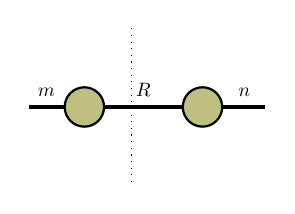
\begin{tikzpicture}[baseline=-0.5ex]
    \tikzset{tensor/.style = {minimum size = 0.5cm,shape = circle,thick,draw=black,inner sep = 0pt}, edge/.style = {thick,line width=.4mm},every loop/.style={}}
    \def\x{6}
    \def\y{0} \node[tensor,fill=green!50!red!50!white] (A) at (\x+1,\y) {$\Ab$};
    \node[tensor,fill=green!50!red!50!white] (B) at (\x+2.5,\y) {$\Bb$};
    \draw[edge] (A) -- (\x+0.3,0) node [midway,above] {\scalebox{0.7}{\dimcolor{$m$}}};
    \draw[edge] (A) -- (B)node [above,midway] {\scalebox{0.7}{\dimcolor{$R$}}};;
    \draw[edge] (B) -- (\x+3.3,\y) node [midway,above] {\scalebox{0.7}{\dimcolor{$n$}}};
    \draw[dotted] (\x+1.6,\y+1) -- (\x+1.6,\y-1);
\end{tikzpicture}\right)\leq R.$$

Now consider the following tensor network representation of a $d_1\times d_2$ matrix:
$$
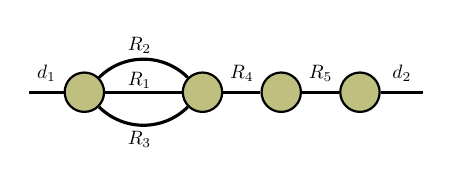
\begin{tikzpicture}[baseline=-0.5ex]
    \tikzset{tensor/.style = {minimum size = 0.5cm,shape = circle,thick,draw=black,inner sep = 0pt}, edge/.style = {thick,line width=.4mm},every loop/.style={}}
    \def\x{6}
    \def\y{0} \node[tensor,fill=green!50!red!50!white] (T) at (\x+1,\y) {$\Tt$};
    \node[tensor,fill=green!50!red!50!white] (A) at (\x+2.5,\y) {$\At$};
    \node[tensor,fill=green!50!red!50!white] (B) at (\x+3.5,\y) {$\Bb$};
      \node[tensor,fill=green!50!red!50!white] (S) at (\x+4.5,\y) {$\Sb$};
    \draw[edge] (T) -- (\x+0.3,\y)node [midway,above] {\scalebox{0.7}{\dimcolor{$d_1$}}};
     \draw[edge] (T) -- (A);
    \draw[edge] (A) -- (B)node [midway,above] {\scalebox{0.7}{\dimcolor{$R_4$}}};
    \draw[edge] (T) to [out=-45,in=-135] (A);
    \draw[edge] (T) to [out=45,in=135] (A);
    \node[draw=none] () at (\x+1.7,\y+0.15) {\scalebox{0.7}{\dimcolor{$R_1$}}};
    \node[draw=none] () at (\x+1.7,\y+0.6) {\scalebox{0.7}{\dimcolor{$R_2$}}};
    \node[draw=none] () at (\x+1.7,\y-0.6) {\scalebox{0.7}{\dimcolor{$R_3$}}};
    \draw[edge](B) -- (S) node [midway,above] {\scalebox{0.7}{\dimcolor{$R_5$}}};
    \draw[edge] (S) -- (\x+5.3,\y) node [midway,above] {\scalebox{0.7}{\dimcolor{$d_2$}}};
    \end{tikzpicture}$$
where $\Tt\in\RR^{d_1\times R_1\times R_2\times R_3}$, $\At\in\RR^{R_1\times R_2\times R_3\times R_4}$, $\Bb\in\RR^{R_4\times R_5}$ and $\Sb\in\RR^{R_5\times d_2}$.
Theorem~\ref{thm: matricization-rank} can for example be used to obtain the upper bounds
$$
\rank\left(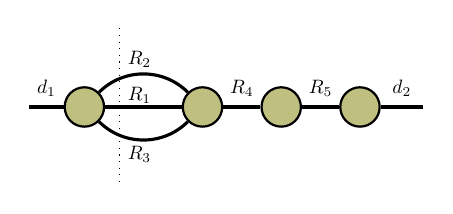
\begin{tikzpicture}[baseline=-0.5ex]
    \tikzset{tensor/.style = {minimum size = 0.5cm,shape = circle,thick,draw=black,inner sep = 0pt}, edge/.style = {thick,line width=.4mm},every loop/.style={}}
    \def\x{6}
    \def\y{0} \node[tensor,fill=green!50!red!50!white] (T) at (\x+1,\y) {$\Tt$};
    \node[tensor,fill=green!50!red!50!white] (A) at (\x+2.5,\y) {$\At$};
    \node[tensor,fill=green!50!red!50!white] (B) at (\x+3.5,\y) {$\Bb$};
      \node[tensor,fill=green!50!red!50!white] (S) at (\x+4.5,\y) {$\Sb$};
    \draw[edge] (T) -- (\x+0.3,\y)node [midway,above] {\scalebox{0.7}{\dimcolor{$d_1$}}};
     \draw[edge] (T) -- (A);
    \draw[edge] (A) -- (B)node [midway,above] {\scalebox{0.7}{\dimcolor{$R_4$}}};
    \draw[edge] (T) to [out=-45,in=-135] (A);
    \draw[edge] (T) to [out=45,in=135] (A);
    \node[draw=none] () at (\x+1.7,\y+0.15) {\scalebox{0.7}{\dimcolor{$R_1$}}};
    \node[draw=none] () at (\x+1.7,\y+0.6) {\scalebox{0.7}{\dimcolor{$R_2$}}};
    \node[draw=none] () at (\x+1.7,\y-0.6) {\scalebox{0.7}{\dimcolor{$R_3$}}};
    \draw[edge](B) -- (S) node [midway,above] {\scalebox{0.7}{\dimcolor{$R_5$}}};
    \draw[edge] (S) -- (\x+5.3,\y) node [midway,above] {\scalebox{0.7}{\dimcolor{$d_2$}}};
    \draw[dotted] (\x+1.45,\y+1) -- (\x+1.45,\y-1);
    \end{tikzpicture}\right)\leq R_1R_2R_3$$
and
$$
\rank
\left(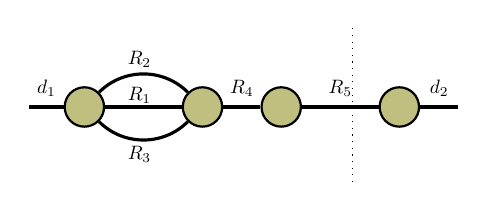
\begin{tikzpicture}[baseline=-0.5ex]
    \tikzset{tensor/.style = {minimum size = 0.5cm,shape = circle,thick,draw=black,inner sep = 0pt}, edge/.style = {thick,line width=.4mm},every loop/.style={}}
    \def\x{6}
    \def\y{0} \node[tensor,fill=green!50!red!50!white] (T) at (\x+1,\y) {$\Tt$};
    \node[tensor,fill=green!50!red!50!white] (A) at (\x+2.5,\y) {$\At$};
    \node[tensor,fill=green!50!red!50!white] (B) at (\x+3.5,\y) {$\Bb$};
      \node[tensor,fill=green!50!red!50!white] (S) at (\x+5,\y) {$\Sb$};
    \draw[edge] (T) -- (\x+0.3,\y)node [midway,above] {\scalebox{0.7}{\dimcolor{$d_1$}}};
     \draw[edge] (T) -- (A);
    \draw[edge] (A) -- (B)node [midway,above] {\scalebox{0.7}{\dimcolor{$R_4$}}};
    \draw[edge] (T) to [out=-45,in=-135] (A);
    \draw[edge] (T) to [out=45,in=135] (A);
    \node[draw=none] () at (\x+1.7,\y+0.15) {\scalebox{0.7}{\dimcolor{$R_1$}}};
    \node[draw=none] () at (\x+1.7,\y+0.6) {\scalebox{0.7}{\dimcolor{$R_2$}}};
    \node[draw=none] () at (\x+1.7,\y-0.6) {\scalebox{0.7}{\dimcolor{$R_3$}}};
    \draw[edge](B) -- (S) node [midway,above] {\scalebox{0.7}{\dimcolor{$R_5$}}};
    \draw[edge] (S) -- (\x+5.75,\y) node [midway,above] {\scalebox{0.7}{\dimcolor{$d_2$}}};
    \draw[dotted] (\x+4.4,\y+1) -- (\x+4.4,\y-1);
    \end{tikzpicture}\right)\leq R_5.
$$
As a final example, let $\Gt\in\RR^{R_1\times\cdots\times R_4}$, $\Ab_1\in\RR^{R_1\times d_1}, \Ab_2\in\RR^{R_2\times d_2},\Ab_3\in\RR^{R_3\times d_3}$ and $\Ab_4\in\RR^{R_4\times d_4}$ and consider the tensor $\T = \Gt \times_1 \Ab_1\times_2 \Ab_2\times_3 \Ab_3\times_4 \Ab_4$. Theorem~\ref{thm: matricization-rank} can be used for example to obtain an upper bound on the rank of the first matricization of $\Tt$:
$$
\rank(\Tt_{(1)}) = 
\rank\left(
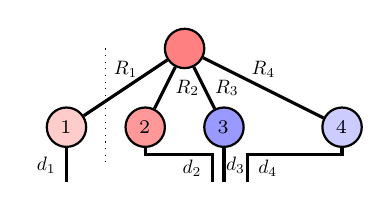
\begin{tikzpicture}[baseline=-0.5ex]
    \tikzset{tensor/.style = {minimum size = 0.5cm,shape = circle,thick,draw=black,inner sep = 0pt}, edge/.style = {thick,line width=.4mm},every loop/.style={}}
    \def\x{6}
    \def\y{0} 
    \node[tensor,fill=red!50!white] (G) at (\x+4.5,\y+1) {$\Gt$};
    \node[tensor,fill=red!20!white] (A_1) at (\x+3,\y){$\Ab_1$};
    \node[tensor,fill=red!40!white] (A_2) at (\x+4,\y){$\Ab_2$};
    \node[tensor, fill=blue!40!white] (A_3) at (\x+5,\y){$\Ab_3$};
    \node[tensor,fill=blue!20!white] (A_4) at (\x+6.5,\y){$\Ab_4$};
    \draw[edge] (G) -- (A_1) node [midway, above] {\scalebox{0.7}{\dimcolor{$R_1$}}};
    \draw[edge] (G) -- (A_2) node [midway, right] {\scalebox{0.7}{\dimcolor{$R_2$}}};
    \draw[edge] (G) -- (A_3) node [midway, right] {\scalebox{0.7}{\dimcolor{$R_3$}}};
    \draw[edge] (G) -- (A_4) node [midway, above] {\scalebox{0.7}{\dimcolor{$R_4$}}};
    \draw[edge] (A_1) -- (\x+3,\y-0.7) node [midway, left] {\scalebox{0.7}{\dimcolor{$d_1$}}};
    \draw[edge] (A_3) -- (\x+5,\y-0.7) node [midway, right=-0.11cm] {\scalebox{0.7}{\dimcolor{$d_3$}}};
    \draw[edge] (A_2) -- (\x+4,\y-0.35) -- (\x+4.85,\y-0.35) -- (\x+4.85,\y-0.7) node [midway, left] {\scalebox{0.7}{\dimcolor{$d_2$}}};
    \draw[edge] (A_4) -- (\x+6.5,\y-0.35) -- (\x+5.30,\y-0.35) -- (\x+5.30,\y-0.7) node [midway, right] {\scalebox{0.7}{\dimcolor{$d_4$}}};
    \draw[dotted](\x+3.5,\y+1)-- (\x+3.5,\y-0.5);
    \end{tikzpicture}\right)\leq R_1.
$$
\paragraph{TN Edges and Sum Tensors.}Let $\T$ be a tensor given as a TN. Any edge in which the TN corresponds to one way to express the tensor as a sum of tensors of the same size as $\T$. This follows directly from the definition of edges in TNs. An edge represents a contraction, which is a sum. We illustrate this concept with examples. First, consider a rank-$R$ factorization of an $m\times n$ matrix. The edge in the TN corresponds to expressing the matrix as a sum of $R$ (rank-one) matrices:  
$$
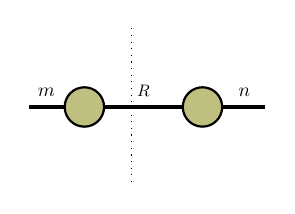
\begin{tikzpicture}[baseline=-0.5ex]
    \tikzset{tensor/.style = {minimum size = 0.5cm,shape = circle,thick,draw=black,inner sep = 0pt}, edge/.style = {thick,line width=.4mm},every loop/.style={}}
    \def\x{6}
    \def\y{0} \node[tensor,fill=green!50!red!50!white] (A) at (\x+1,\y) {$\Ab$};
    \node[tensor,fill=green!50!red!50!white] (B) at (\x+2.5,\y) {$\Bb$};
    \draw[edge] (A) -- (\x+0.3,0) node [midway,above] {\scalebox{0.7}{\dimcolor{$m$}}};
    \draw[edge] (A) -- (B)node [above,midway] {\scalebox{0.6}{\dimcolor{$R$}}};;
    \draw[edge] (B) -- (\x+3.3,\y) node [midway,above] {\scalebox{0.7}{\dimcolor{$n$}}};
    \draw[dotted] (\x+1.6,\y+1) -- (\x+1.6,\y-1);
\end{tikzpicture}
= 
\sum_{r=1}^R
\begin{tikzpicture}[baseline=-0.5ex]
    \tikzset{tensor/.style = {minimum size = 0.5cm,shape = circle,thick,draw=black,inner sep = 0pt}, edge/.style = {thick,line width=.4mm},every loop/.style={}}
    \def\x{6}
    \def\y{0} \node[tensor,fill=green!50!red!50!white] (A) at (\x+1,\y) {$\Ab$};
    \node[tensor,fill=green!50!red!50!white] (B) at (\x+2.5,\y) {$\Bb$};
    \draw[edge] (A) -- (\x+0.3,0) node [midway,above] {\scalebox{0.7}{\dimcolor{$m$}}};
    \draw[edge] (A) -- (\x+1.5,\y) node [pos=1.5] {\scalebox{0.7}{\indcolor{$r$}}};
    \draw[edge] (B) -- (\x+3.3,\y) node [midway,above] {\scalebox{0.7}{\dimcolor{$n$}}};
    \draw[edge](B) -- (\x+2,\y)node [pos=1.4] {\scalebox{0.7}{\indcolor{$r$}}};
\end{tikzpicture}
= \sum_{r=1}^R \Ab_{:,r} \Bb_{r,:} = \sum_{r=1}^R \ab_r \outprod \bb_r,
$$
where $\ab_r$ are the columns of $\Ab\in\RR^{m\times R}$ and $\bb_r$ are the rows of $\Bb\in\RR^{R\times n}$.

Similarly, the unique edge in the TN representing the trace of a matrix corresponds to expressing the TN~(which is a scalar) as a sum of scalars~(the diagonal entries of the matrix), let $\Ab\in\RR^{d\times d}$:
$$\begin{tikzpicture}[baseline=\baseline]
    \tikzset{tensor/.style = {minimum size = 0.5cm,shape = circle,thick,draw=black,inner sep = 0pt}, edge/.style = {thick,line width=.4mm},every loop/.style={}}
    \def\y{0}
    \def\x{0}
    \node[tensor,fill=red!50!white] (A) at (\x,\y+0.2){\scalebox{0.85}{$\Ab$}};
    \draw[edge] (A) to [out=-20,in=-160, distance=1.35cm] (A);
    \draw[dotted] (\x-0.15,\y-0.1) -- (\x-0.15,\y-0.8);
    \node[draw=none] () at (\x,\y-0.4) {\scalebox{0.7}{\dimcolor{$d$}}};
\end{tikzpicture}\hspace{-0.7cm}
=
\sum_{i=1}^d\left(
\begin{tikzpicture}[baseline=\baseline]
    \tikzset{tensor/.style = {minimum size = 0.5cm,shape = circle,thick,draw=black,inner sep = 0pt}, edge/.style = {thick,line width=.4mm},every loop/.style={}}
    \def\y{0}
    \def\x{0}
    \node[tensor,fill=red!50!white] (A) at (\x,\y){\scalebox{0.85}{$\Ab$}};
     \draw[edge] (\x-0.25,\y) to [out=110,in=60, distance=0.1cm] (\x-0.6,\y-0.2);    
    \draw[edge] (\x+0.25,\y) to [out=110,in=60, distance=0.1cm] (\x+0.6,\y-0.2); 
    \node[draw=none] () at (\x+0.7,\y-0.25) {\scalebox{0.7}{\indcolor{$i$}}};
    \node[draw=none] () at (\x-0.7,\y-0.25) {\scalebox{0.7}{\indcolor{$i$}}};
    \end{tikzpicture}\right)=\sum_{i=1}^d\Ab_{ii}.
    $$
Consider now a more interesting example:
$$\begin{tikzpicture}[baseline=\baseline]
    \tikzset{tensor/.style = {minimum size = 0.5cm,shape = circle,thick,draw=black,inner sep = 0pt}, edge/.style = {thick,line width=.4mm},every loop/.style={}}
    \def\y{0}
    \def\x{0}
    \node[tensor,fill=red!50!white] (A) at (\x,\y+0.5){\scalebox{0.85}{$\Ab$}};
    \node[tensor,fill=red!50!white] (B) at (\x,\y-0.5){\scalebox{0.85}{$\Bb$}};
    \draw[edge](A)--(B)node [midway, right] {\scalebox{0.7}{\dimcolor{$R$}}};
    \draw[edge](A) -- (\x+0.5,\y+0.5)--(\x+0.5,\y)--(\x+1,\y)node [midway, above] {\scalebox{0.7}{\dimcolor{$n$}}};
    \draw[edge](A) -- (\x-0.5,\y+0.5)--(\x-0.5,\y)--(\x-1,\y)node [midway, above] {\scalebox{0.7}{\dimcolor{$m$}}};
    \draw[edge](B) -- (\x+0.5,\y-0.5)--(\x+0.5,\y-0.1)--(\x+1,\y-0.1)node [midway, below] {\scalebox{0.7}{\dimcolor{$q$}}};
    \draw[edge](B) -- (\x-0.5,\y-0.5)--(\x-0.5,\y-0.1)--(\x-1,\y-0.1)node [midway, below] {\scalebox{0.7}{\dimcolor{$p$}}};
    \end{tikzpicture}.$$
The edge in this TN corresponds to a way to express the matrix represented by the TN as a sum of matrices:
$$\begin{tikzpicture}[baseline=\baseline]
    \tikzset{tensor/.style = {minimum size = 0.5cm,shape = circle,thick,draw=black,inner sep = 0pt}, edge/.style = {thick,line width=.4mm},every loop/.style={}}
    \def\y{0}
    \def\x{0}
    \node[tensor,fill=red!50!white] (A) at (\x,\y+0.5){\scalebox{0.85}{$\Ab$}};
    \node[tensor,fill=red!50!white] (B) at (\x,\y-0.5){\scalebox{0.85}{$\Bb$}};
    \draw[edge](A)--(B)node [midway, right] {\scalebox{0.7}{\dimcolor{$R$}}};
    \draw[edge](A) -- (\x+0.5,\y+0.5)--(\x+0.5,\y)--(\x+1,\y)node [midway, above] {\scalebox{0.7}{\dimcolor{$n$}}};
    \draw[edge](A) -- (\x-0.5,\y+0.5)--(\x-0.5,\y)--(\x-1,\y)node [midway, above] {\scalebox{0.7}{\dimcolor{$m$}}};
    \draw[edge](B) -- (\x+0.5,\y-0.5)--(\x+0.5,\y-0.1)--(\x+1,\y-0.1)node [midway, below] {\scalebox{0.7}{\dimcolor{$q$}}};
    \draw[edge](B) -- (\x-0.5,\y-0.5)--(\x-0.5,\y-0.1)--(\x-1,\y-0.1)node [midway, below] {\scalebox{0.7}{\dimcolor{$p$}}};
    \draw[dotted](\x+0.35,\y+0.15) -- (\x-0.35,\y+0.15);
    \end{tikzpicture}
    =
    \sum_{r=1}^R\begin{tikzpicture}[baseline=\baseline]
    \tikzset{tensor/.style = {minimum size = 0.5cm,shape = circle,thick,draw=black,inner sep = 0pt}, edge/.style = {thick,line width=.4mm},every loop/.style={}}
    \def\y{0}
    \def\x{0}
    \node[tensor,fill=red!50!white] (A) at (\x,\y+1){\scalebox{0.85}{$\Ab$}};
    \node[tensor,fill=red!50!white] (B) at (\x,\y-1){\scalebox{0.85}{$\Bb$}};
    \draw[edge](A) -- (\x,\y+0.45)node [pos=1.4]{\scalebox{0.7}{\indcolor{$r$}}};
    \draw[edge](B) -- (\x,\y-0.45)node [pos=1.3]{\scalebox{0.7}{\indcolor{$r$}}};
    \draw[edge](A) -- (\x+0.5,\y+1)--(\x+0.5,\y)--(\x+1,\y)node [midway, above] {\scalebox{0.7}{\dimcolor{$n$}}};
    \draw[edge](A) -- (\x-0.5,\y+1)--(\x-0.5,\y)--(\x-1,\y)node [midway, above] {\scalebox{0.7}{\dimcolor{$m$}}};
    \draw[edge](B) -- (\x+0.5,\y-1)--(\x+0.5,\y-0.1)--(\x+1,\y-0.1)node [midway, below] {\scalebox{0.7}{\dimcolor{$q$}}};
    \draw[edge](B) -- (\x-0.5,\y-1)--(\x-0.5,\y-0.1)--(\x-1,\y-0.1)node [midway, below] {\scalebox{0.7}{\dimcolor{$p$}}};
    \end{tikzpicture}
    =
    \sum_{r=1}^R\Ab_r\kron\Bb_r.$$
We recognize here that this TN corresponds to a sum of Kronecker products! 
\paragraph{Tensors, Multilinear Maps and Polynomials.}
We can think of tensors as \emph{representations of multi-linear maps}, in exactly the same sense that matrices represent linear maps. Recall that a matrix $\Ab\in\RR^{m\times n}$ represents a linear map $\RR^n\to\RR^m$ via $\xb\mapsto \Ab\xb$. In tensor network notation, this is simply
$$
\yb = \Ab\xb
=
\begin{tikzpicture}[baseline=-0.5ex]
    \tikzset{tensor/.style = {minimum size = 0.5cm,shape = circle,thick,draw=black,inner sep = 0pt},
             edge/.style   = {thick,line width=.4mm},every loop/.style={}}
    \def\x{0}\def\y{0}
    \node[tensor,fill=red!50!white] (A) at (\x,\y){$\Ab$};
    \node[tensor,fill=blue!20!white] (x) at (\x+1,\y){$\xb$};
    \draw[edge] (A) -- (x) node [midway,above]{\scalebox{0.7}{\dimcolor{$n$}}};
    \draw[edge] (A) -- (\x-1,\y) node [midway,above]{\scalebox{0.7}{\dimcolor{$m$}}};
\end{tikzpicture}
\in\RR^{m}.
$$
Linearity means that $\Ab(\alpha \xb+\beta \zb)=\alpha \Ab\xb+\beta \Ab\zb$ for all $\alpha,\beta\in\RR$ and $\xb,\zb\in\RR^n$. A tensor is the natural generalization when the map is linear \emph{in several arguments separately}. Concretely, an order-$N$ tensor $\Tt\in\RR^{d_1\times\cdots\times d_N}$ defines a map that takes $N$ input vectors and returns a scalar by contracting along all modes:
$$
f(\xb^{(1)},\dots,\xb^{(N)})
:= \langle \Tt,\ \xb^{(1)}\outprod \cdots \outprod \xb^{(N)}\rangle
=
\sum_{i_1=1}^{d_1}\cdots\sum_{i_N=1}^{d_N}\Tt_{i_1\cdots i_N}\,\xb^{(1)}_{i_1}\cdots \xb^{(N)}_{i_N}.
$$
This map is \emph{multi-linear}: it is linear in each $\xb^{(k)}$ when the other vectors are fixed. In tensor network diagrams, this is simply
\[
f(\ab,\bb,\dots,\zb)
=
\begin{tikzpicture}[baseline=2ex]
    \tikzset{tensor/.style = {minimum size = 0.5cm,shape = circle,thick,draw=black,inner sep = 0pt},
             edge/.style   = {thick,line width=.4mm},
             every loop/.style={}}
    \def\x{0}\def\y{0}

    \node[tensor,fill=green!50!red!50!white] (T) at (\x,\y+0.8){$\Tt$};

    \node[tensor,fill=blue!20!white] (a) at (\x-1.2,\y){$\ab$};
    \node[tensor,fill=blue!20!white] (b) at (\x-0.5,\y){$\bb$};
    \node[draw=none] (dots) at (\x+0.5,\y){$\cdots$};
    \node[tensor,fill=blue!20!white] (z) at (\x+1.2,\y){$\zb$};

    \draw[edge] (T) -- (a) node [near end,above]{\scalebox{0.7}{\dimcolor{$d_1\ $}}};
    \draw[edge] (T) -- (b) node [near end,right]{\scalebox{0.7}{\dimcolor{$d_2$}}};
    \draw[edge] (T) -- (z) node [near end,above]{\scalebox{0.7}{\dimcolor{$d_N$}}};
\end{tikzpicture}
\in\RR,
\]
where $\ab, \bb,\cdots,\zb\in\RR^d$.
If we leave one leg open, we obtain a \emph{vector-valued} multi-linear map. For instance, if $\Tt\in\RR^{d_1\times\cdots\times d_N \times p}$, contracting all modes except the last defines a multi-linear map whose output is a vector of dimension $p$:
$$
f(\ab,\bb,\dots,\zb)
=
\begin{tikzpicture}[baseline=2ex]
    \tikzset{tensor/.style = {minimum size = 0.5cm,shape = circle,thick,draw=black,inner sep = 0pt},
             edge/.style   = {thick,line width=.4mm},
             every loop/.style={}}
    \def\x{0}\def\y{0}

    \node[tensor,fill=green!50!red!50!white] (T) at (\x,\y+0.8){$\Tt$};

    \node[tensor,fill=blue!20!white] (a) at (\x-1.2,\y){$\ab$};
    \node[tensor,fill=blue!20!white] (b) at (\x-0.5,\y){$\bb$};
    \node[draw=none] (dots) at (\x+0.5,\y){$\cdots$};
    \node[tensor,fill=blue!20!white] (z) at (\x+1.2,\y){$\zb$};

    \draw[edge] (T) -- (a) node [near end,above]{\scalebox{0.7}{\dimcolor{$d_1\ $}}};
    \draw[edge] (T) -- (b) node [near end,right]{\scalebox{0.7}{\dimcolor{$d_2$}}};
    \draw[edge] (T) -- (z) node [near end,above]{\scalebox{0.7}{\dimcolor{$d_N$}}};
    \draw[edge] (T) -- (\x,\y+1.6) node [midway,right]{\scalebox{0.7}{\dimcolor{$p$}}};
\end{tikzpicture}
\in\RR^p.
$$

\vspace{0.2cm}
\noindent
This immediately connects the tensors to \emph{multivariate polynomials}. The scalar map
\[
f(\xb^{(1)},\dots,\xb^{(N)})=\sum_{i_1,\dots,i_N}\Tt_{i_1\cdots i_N}\,\xb^{(1)}_{i_1}\cdots \xb^{(N)}_{i_N},
\]
is a polynomial in the entries of the vectors and is \emph{multi-linear}: every variable appears with degree at most one (when viewed in each block of variables $\xb^{(k)}$). In the important special case where all inputs are the \emph{same} vector $\xb\in\RR^{d}$ and $\Tt\in\RR^{d\times\cdots\times d}$ has $N$ modes, the  contraction
\[
\begin{tikzpicture}[baseline=2ex]
    \tikzset{tensor/.style = {minimum size = 0.5cm,shape = circle,thick,draw=black,inner sep = 0pt},
             edge/.style   = {thick,line width=.4mm},
             every loop/.style={}}
    \def\x{0}\def\y{0}

    \node[tensor,fill=green!50!red!50!white] (T) at (\x,\y+0.8){$\Tt$};

    \node[tensor,fill=blue!20!white] (a) at (\x-1.2,\y){$\xb$};
    \node[tensor,fill=blue!20!white] (b) at (\x-0.5,\y){$\xb$};
    \node[draw=none] (dots) at (\x+0.5,\y){$\cdots$};
    \node[tensor,fill=blue!20!white] (z) at (\x+1.2,\y){$\xb$};

    \draw[edge] (T) -- (a) node [midway,left]{\scalebox{0.7}{\dimcolor{$d\ $}}};
    \draw[edge] (T) -- (b) node [near end,right]{\scalebox{0.7}{\dimcolor{$d$}}};
    \draw[edge] (T) -- (z) node [midway,right]{\scalebox{0.7}{\dimcolor{$\ d$}}};
\end{tikzpicture}
= \Tt \ttm{1}\xb \ttm{2}\xb \cdots \ttm{N}\xb
=
\sum_{i_1,\dots,i_N}\Tt_{i_1\cdots i_N}\,\xb_{i_1}\cdots \xb_{i_N} \in \RR.
\]
is a \emph{homogeneous} multivariate polynomial of degree $N$ (every monomial has total degree exactly $N$). The tensor entries are precisely the coefficients of this polynomial in the monomial basis $(\xb_{i_1}\cdots \xb_{i_N})_{i_1,\cdots,i_N}$.

If instead we contract an order-$(N+1)$ tensor $\Tt\in\RR^{ d\times\cdots\times d \times p}$ with $N$ copies of $\xb\in\RR^d$, leaving the last leg free, we obtain a vector-valued homogeneous polynomial map $\RR^d\to\RR^m$:
\[
p(\xb) = \Tt \ttm{1}\xb \ttm{2}\xb\cdots \ttm{N}\xb \in\RR^{p}.
\]

\vspace{0.2cm}
\noindent
Finally, \emph{non-homogeneous} polynomials can be obtained using a simple trick: \emph{append a constant $1$ to the input vector}. Let $\xb\in\RR^d$ and define the augmented vector $\tilde{\xb} =\begin{bmatrix}\xb\\1\end{bmatrix}\in\RR^{d+1}$. If $\widetilde{\Tt}\in\RR^{(d+1)\times\cdots\times(d+1)}$ is an order-$N$ tensor, then
\[
\tilde{p}(\xb)
:=
\widetilde{\Tt} \ttm{1}\tilde{\xb}\ttm{2}\tilde{\xb}\cdots\ttm{N}\tilde{\xb},
\]
is a polynomial in $\xb$ of degree at most $N$ (some factors can pick the last coordinate, which is the constant $1$, thereby lowering the degree of the corresponding monomials). In other words, a single homogeneous tensor polynomial in the augmented variables $(x_1,\dots,x_d,1)$ compactly represents a general multivariate polynomial in $(x_1,\dots,x_d)$. This viewpoint is especially useful in practice: it lets us treat bias terms and lower-degree interactions using the same contraction machinery as the homogeneous case, simply by adding one extra dimension to each mode and fixing it to $1$.  
